\documentclass[journal]{IEEEtran}
\usepackage[english]{babel}
\usepackage{%
  float,
  amssymb,
  amsmath,
  fullpage,
  indentfirst,
  mathrsfs,
  hyperref,
  empheq,
  mathtools,
  enumerate,
  amsthm,
  thmtools,
  cite,
  multicol,
  mathtools,
  cuted,
  ../sty/widetext % chktex 26
}
\usepackage[shortlabels]{enumitem}

% Figures
\newcommand{\figurepath}{../fig}
\newcommand{\bibstylepath}{../sty/IEEEtran}
\newcommand{\bibsourcepath}{../bib/ieee-access-2017}

% Theorem styles
\declaretheoremstyle[
  headfont=\bfseries,
  notebraces={}{},
  notefont=\bfseries,
  bodyfont=\itshape,
  headpunct={},
  headformat={\hspace{0.0in}\makebox[0.65in][l]{\NAME\ \NUMBER\ }{\NOTE}}\hspace{0.1in}
]{thm-style}

\declaretheoremstyle[
  headfont=\bfseries,
  notebraces={}{},
  notefont=\bfseries,
  bodyfont=\itshape,
  headpunct={},
  headformat={\hspace{0.0in}\makebox[0.65in][l]{\NAME\ \NUMBER\ }{\NOTE}}\hspace{0.1in}
]{lem-style}

\declaretheoremstyle[
  headfont=\bfseries,
  notebraces={}{},
  notefont=\bfseries,
  bodyfont=\itshape,
  headpunct={},
  headformat={\NAME\ \NUMBER\ }
]{cor-style}

\declaretheoremstyle[
  headfont=\scshape,
  notefont=\itshape,
  bodyfont=\normalfont,
  headpunct=\relax,
  headformat={\makebox[0.5in][r]{\NAME\ }\NOTE},
]{prf-style}

\declaretheoremstyle[
  headfont=\bfseries,
  notebraces={}{},
  notefont=\bfseries,
  headpunct={},
  headformat={\NAME\ \NUMBER\ }{\NOTE}
]{rem-style}

% Relax
\let\proof\relax
\let\endproof\relax

% Declare theorems
\declaretheorem[style=thm-style,numbered=yes,name=Theorem]{thm-dan}
\declaretheorem[style=lem-style,numbered=yes,name=Lemma]{lem-dan}
\declaretheorem[style=cor-style,numbered=yes,name=Corollary]{cor-dan}
\declaretheorem[style=prf-style,name=Proof,qed=\qedsymbol]{proof-dan}
\declaretheorem[style=rem-style,numbered=yes,name=Remark]{rem-dan}

% Bold symbols in section headings
\makeatletter
\g@addto@macro\bfseries{\boldmath}
\makeatother

\newtheoremstyle{innercustomthm}
  {\topsep}% measure of space to leave above the theorem. E.g.: 3pt
  {\topsep}% measure of space to leave below the theorem. E.g.: 3pt
  {\itshape}% name of font to use in the body of the theorem
  {0pt}% measure of space to indent
  {\bfseries}% name of head font
  {}% punctuation between head and body
  {2pt}% space after theorem head; " " = normal interword space
  {\thmname{#1}\thmnumber{#2}\thmnote{(#3)}}
\theoremstyle{innercustomthm}

% Assumption
\newtheorem{innercustomthm}{Assumption}
\newenvironment{ass-dan}[1]
{\renewcommand\theinnercustomthm{#1}\innercustomthm\normalfont}
{\endinnercustomthm}

\begin{document}

  \title{Sequential Loop Closure Based Adaptive Output Feedback}

  \author{Daniel~P.~Wiese,~\IEEEmembership{Student Member,~IEEE,}
          Anuradha~M.~Annaswamy,~\IEEEmembership{Fellow,~IEEE,}
          Jonathan~A.~Muse,~\IEEEmembership{Fellow,~IEEE,}
          Michael~A.~Bolender,
          and~Eugene~Lavretksy,~\IEEEmembership{Fellow,~IEEE}%
  \thanks{D.P. Wiese and A.M. Annaswamy are with the Department of Mechanical Engineering, Massachusetts Institute of Technology, Cambridge, MA 02139 USA (e-mail: dpwiese@mit.edu; aanna@mit.edu).}%
  \thanks{J.A. Muse and M.A. Bolender are with the Air Force Research Laboratory (Air Vehicles Directorate), Control Design and Analysis Branch, 2210 Eighth Street, WPAFB, OH 45433.}%
  \thanks{E. Lavretsky is with the Phantom Works Department, Boeing Company, Huntington Beach, CA 92647 USA (e-mail: eugene.lavretsky@boeing.com)}}

  \maketitle

  \begin{abstract}
    This paper presents a new, systematic method of synthesizing an output feedback adaptive controller for a class of uncertain, non-square multi-input/multi-output systems.
    The control design process consists of first designing an inner-loop controller for a reduced order plant model to enforce command tracking of selected inner-loop variables, with an adaptive element used to accommodate parametric uncertainties in the plant.
    Once this inner-loop control design is complete, an outer-loop is then designed which prescribes the inner-loop commands to enforce command tracking of selected outer-loop variables.

    The main challenge that needs to be addressed when designing the inner-loop controller is the determination of a corresponding square and strictly positive real transfer function.
    This is accomplished by appropriate selection of two gain matrices that allow the realization of such a transfer function, thereby allowing a globally stable adaptive output feedback law to be generated.
    The outer-loop controller is designed around the plant with existing adaptive inner-loop controller such that global stability of the closed-loop system is guaranteed.
    The design of the outer-loop uses components of a closed-loop reference model in a judicious manner which enables a modular approach, without requiring any re-design of the inner-loop controller.
    In addition, this architecture facilitates the use of an additional state-limiter to enforce desired limits on the state variables.

    A numerical example based on a scramjet powered, generic hypersonic vehicle model is presented, demonstrating the efficacy of the proposed control design.
  \end{abstract}

  \begin{IEEEkeywords}
    \bfseries
    Adaptive control.
  \end{IEEEkeywords}

  \IEEEpeerreviewmaketitle%

  \section{Introduction}\label{sec.intro}

  \IEEEPARstart{D}{ividing} a control system into hierarchical structure with inner and outer-loops has many benefits, both in aerospace and other control applications.
  Significant knowledge exists around how to design many of the inner-loop controllers that provide stability and robustness to the closed-loop system, and the limiting of inner-loop commands is facilitated by this hierarchical structure in which these commands are explicitly calculated by the outer-loop.

  Obtaining accurate values of the system parameters can be challenging, thus making the process of designing a stabilizing controller more challenging as well.
  This has led to an increased use of adaptive techniques to solve control problems, with great success\ \cite{astrom.feedback.1987, lavretskywise.book.2013}.
  However, many such adaptive controllers have previously focused only on the problem of inner-loop control\ \cite{mcfarland.autopilot.1996, qu.gnc.2013, wiese.adaptive.2013, wiese.gnc.2015, wiese.jgcd.2015, wise.munition.2005, wise.autopilot.2008}, enabling the design of lower order controllers to provide stability in the presence of uncertainties.
  In these and many other cases outer-loops were typically not designed.
  In aerospace applications, the design of the guidance laws around vehicles with adaptive inner loops is typically accomplished using ad-hoc methods, with stability and performance of the closed-loop system only verified through simulation.

  An alternative to the multi-loop design approach described above is to use a higher order model to represent the vehicle dynamics, and design guidance and control laws simultaneously.
  The result is a more complex controller with a greater number of integrators and adaptive parameters.
  In Ref.\ \cite{gibson.adaptive.2008} an adaptive controller was designed for a linear system which represents the longitudinal dynamics of a hypersonic vehicle.
  The controller used feedback from all five state variables to each of the three inputs, with additional feed forward terms, resulting in 24 adaptive parameters.

  Other approaches have used sequential loop closure on higher order nonlinear models.
  In Ref.\ \cite{fiorentini.canard.2008} the non-minimum phase dynamics typically associated with the transfer function from an aircraft's elevator input to the altitude were overcome by the addition of a canard, which would be practically impossible to implement on a hypersonic vehicle due to the effects that aerodynamic heating would have on such a forward control surface.
  In Ref.\ \cite{fiorentini.nmp.2009} a canard is no longer used, and the resulting unstable zero dynamics associated with regulating flight path angle using the elevator input are overcome using a non-adaptive dynamic inversion controller with a low gain outer loop and saturation functions.
  Reference\ \cite{bodson.autopilot.2003} uses an adaptive dynamic inversion inner-loop control law, with a parameter identification algorithm which requires the state derivative be measurable.
  The outer-loop is closed using sequential loop closure, but no stability proof is provided to ensure stability of the overall closed-loop system.

  The main contribution of this paper is the design of an outer-loop controller which prescribes commands to an inner-loop adaptive controller such as those described in Refs.\ \cite{lavretskywise.book.2013, qu.gnc.2013, wiese.adaptive.2013, wiese.gnc.2015, wiese.jgcd.2015}.
  Specifically, this outer-loop controller does not require the inner-loop controller be redesigned, guarantees stability of the closed-loop system, and incorporates a state limiter, allowing the inner and outer-loop command signals to be modified as necessary to limit the evolution of the state trajectories to within a certain prescribed region within the state space.

  In the following section the control problem is formulated with a general structure applicable to a wide class of systems.

  \section{Preliminaries}

  The following well-known lemma gives necessary and sufficient conditions to ensure that the system $(A,B,C,0)$ is strictly positive real (SPR).
  \begin{lem-dan}[(Kalman-Yakubovic)]\label{lem.KY}
    Given the strictly proper transfer matrix $G(s)$ with stabilizable and detectable realization $(A,B,C,0)$, where $A\in\mathbb{R}^{n\times n}$ is asymptotically stable, $B\in\mathbb{R}^{n\times m}$ and $C\in\mathbb{R}^{m\times n}$, then $G(s)$ is SPR if and only if there exists a $P=P^{\top}>0$ such that
    \begin{align}
      \label{eqn.lyapal2}
      A^{\top}P+PA&<0 \\
      \label{eqn.pbc}
      PB&=C^{\top}
    \end{align}
  \end{lem-dan}

  \begin{proof-dan}
    The proof can be found in Ref.\ \cite{narendra.frequency.1973}.
  \end{proof-dan}

  \begin{cor-dan}
    There exists a matrix $P=P^{\top}>0$ that satisfies\ \eqref{eqn.pbc} if and only if
    \begin{equation}
      \label{eqn.cbeqcbt}
      CB=(CB)^{\top}>0
    \end{equation}
    Furthermore, when\ \eqref{eqn.cbeqcbt} holds, all solutions of\ \eqref{eqn.pbc} are given by
    \begin{equation}
      \label{eqn.Psolutions}
      P=C^{\top}(CB)^{-\top}C+B^{\perp}XB^{\perp\top}
    \end{equation}
    where $X=X^{\top}>0$ is arbitrary and $B^{\perp}\in\mathbb{R}^{n\times(n-m)}$.
  \end{cor-dan}

  \begin{proof-dan}
    The proof can be found in Ref.\ \cite{huang.designspr.1999}.
  \end{proof-dan}

  \begin{lem-dan}[(Matrix Elimination)]\label{lem.elimination}
    Given
    \begin{equation}
      \label{eqn:ineqprove}
      G+C^{\top}L^{\top}P+PLC<0
    \end{equation}
    where $G\in\mathbb{R}^{n\times n}$, $C\in\mathbb{R}^{p\times n}$, and $P=P^{\top}\in\mathbb{R}^{n\times n}$ is full rank, an $L\in\mathbb{R}^{n\times p}$ exists which satisfies\ \eqref{eqn:ineqprove} if and only if the following inequality holds
    \begin{equation*}
      C^{\top\perp\top}GC^{\top\perp}<0
    \end{equation*}
    where $C^{\top\perp}\in\mathbb{R}^{n\times(n-p)}$ satisfies $CC^{\top\perp}=0$.
  \end{lem-dan}

  \begin{proof-dan}
    The proof can be found in Ref.\ \cite{boyd.lmibook.1994}.
  \end{proof-dan}

  \section{Control Problem Formulation}\label{sec.analysisandclassical}

  Consider the following uncertain linear time-invariant system

  {%
    \small
    \setlength{\abovedisplayskip}{0pt}
    \setlength{\belowdisplayskip}{6pt}
    \setlength{\abovedisplayshortskip}{3pt}
    \setlength{\belowdisplayshortskip}{3pt}
    \begin{align}
      \label{eqn.wholeSystemUncertain}
      \begin{bmatrix}
        \dot{x}_{p}(t) \\
        \dot{x}_{g}(t)
      \end{bmatrix}
      &=
      \begin{bmatrix}
        A_{p}+B_{p}\Psi_{p}^{\top} & B_{gd} \\
        B_{gp} & A_{g}
      \end{bmatrix}
      \begin{bmatrix}
        x_{p}(t) \\
        x_{g}(t)
      \end{bmatrix}
      +
      \begin{bmatrix}
        B_{p}\Lambda \\
        0
      \end{bmatrix}
      u(t) \nonumber \\
      \begin{bmatrix}
        y_{p}(t) \\
        y_{g}(t)
      \end{bmatrix}
      &=
      \begin{bmatrix}
        C_{p} & 0 \\
        0 & C_{g}
      \end{bmatrix}
      \begin{bmatrix}
        x_{p}(t) \\
        x_{g}(t)
      \end{bmatrix} \\
      \begin{bmatrix}
        z_{p}(t) \\
        z_{g}(t)
      \end{bmatrix}
      &=
      \begin{bmatrix}
        C_{pz}+D_{pz}\Psi_{p}^{\top} & 0 \\
        0 & C_{gz}
      \end{bmatrix}
      \begin{bmatrix}
        x_{p}(t) \\
        x_{g}(t)
      \end{bmatrix}
      +
      \begin{bmatrix}
        D_{pz}\Lambda \\
        0
      \end{bmatrix}
      u(t) \nonumber
    \end{align}
  }%
  where $A_{p}\in\mathbb{R}^{n_{p}\times n_{p}}$, $A_{g}\in\mathbb{R}^{n_{g}\times n_{g}}$, $B_{p}\in\mathbb{R}^{n_{p}\times m}$, $B_{gp}\in\mathbb{R}^{n_{g}\times n_{p}}$, $B_{gd}\in\mathbb{R}^{n_{p}\times n_{g}}$, $C_{p}\in\mathbb{R}^{\ell_{p} \times n_{p}}$, $C_{g}\in\mathbb{R}^{\ell_{g}\times n_{g}}$, $C_{pz}\in\mathbb{R}^{n_{ep}\times n_{p}}$, $C_{gz}\in\mathbb{R}^{n_{eg}\times n_{g}}$, and $D_{pz}\in\mathbb{R}^{n_{ep}\times m}$ are \textit{known} matrices.
  The nonsingular matrix $\Lambda\in\mathbb{R}^{m\times m}$, and $\Psi_{p}\in\mathbb{R}^{n_{p}\times m}$, which represents constant matched uncertainty weights that enter the system through the columns of $B_{p}$, are \textit{unknown}.
  The \textit{measured outputs} are given by $y_{p}(t)$ and $y_{g}(t)$, and the \textit{regulated outputs} $z_{p}(t)$ and $z_{g}(t)$ correspond to particular outputs for which tracking of command signals $z_{p,\text{cmd}}(t)$ and $z_{g,\text{cmd}}^{\prime}(t)$, respectively, is desired.
  The number of regulated outputs cannot exceed the number of inputs, that is $n_{ep}\leq m$.
  Ultimately, the \textit{control goal} is to design $u(t)$ in\ \eqref{eqn.wholeSystemUncertain} so that $z_{g}(t)$ tracks $z_{g,\text{cmd}}^{\prime}(t)$.

  \section{Inner Loop Control Design}\label{sec.InnerLoopControlDesign}

  For systems represented by\ \eqref{eqn.wholeSystemUncertain}, $x_{p}$ represents the inner-loop, and $x_{g}$ the outer-loop state variables.
  An inner-loop controller is designed by neglecting the outer-loop variables by assuming $B_{gd}=0$ giving
  {%
    \small
    \setlength{\belowdisplayskip}{-8pt}
    \begin{align}
      \label{eqn.innerLoopDynamicsUncertain}
      \dot{x}_{p}(t) &= A_{p}x_{p}(t) + B_{p}\bigr(\Lambda u(t) + \Psi_{p}^{\top}x_{p}(t)\bigr)+B_{gd}x_{g}(t) \nonumber \\
      y_{p}(t) &= C_{p}x_{p}(t) \\
      z_{p}(t) &= C_{pz}x_{p}(t) + D_{pz}\bigr(\Lambda u(t) + \Psi_{p}^{\top}x_{p}(t)\bigr) \nonumber \\ \nonumber
    \end{align}
  }%

  To satisfy the control goal, the problem is restated as: first design the input $u(t)$ in\ \eqref{eqn.innerLoopDynamicsUncertain} so that $z_{p}(t)$ tracks $z_{p,\text{cmd}}(t)$ with bounded errors in the presence of the uncertainties $\Lambda$ and $\Psi_{p}$.
  Then re-introduce the outer-loop dynamics and then design $z_{p,\text{cmd}}(t)$ so that $z_{g}(t)$ tracks $z_{g,\text{cmd}}^{\prime}(t)$.
  We make the following assumptions about the form of the system represented in\ \eqref{eqn.innerLoopDynamicsUncertain}.

  \begin{ass-dan}{1} $\;$\label{ass.plant}
    \begin{enumerate}[\Alph{enumi}), ref=\Alph{enumi}] % chktex 9 chktex 10
      \item{$(A_{p},B_{p})$ is controllable.\label{ass.p.cont}}
      \item{$(A_{p},C_{p})$ is observable.\label{ass.p.obsv}}
      \item{$B_{p}$, $C_{p}$, and $C_{p}B_{p}$ are full rank.\label{ass.p.rank}}
      \item{Any finite transmission zeros of $(A_{p},B_{p},C_{p},0)$ are strictly stable, and the rank of the following matrix is full\label{ass.p.tzero}}
      \begin{equation*}
        \text{rank}\left(
        \begin{bmatrix}
          A_{p} & B_{p} \\
          C_{pz} & D_{pz}
        \end{bmatrix}\right)
        =n_{p}+n_{ep}
      \end{equation*}
      \item{%
        \begin{enumerate}[(\alph{enumii}), ref=\alph{enumii}] % chktex 9 chktex 10
          \item{$\Lambda$ is nonsingular and diagonal with entries of known sign\label{ass.p.unc.lambda}}
          \item{$\|\Psi_{p}\|_{2}<\Psi_{\text{max}}<\infty$, where $\Psi_{\text{max}}$ is known\label{ass.p.unc.wp}}
        \end{enumerate}\label{ass.p.unc}
      }
    \end{enumerate}
  \end{ass-dan}

  In order to facilitate command tracking, integral action is introduced, and for this purpose an additional state $x_{e}(t)$ is defined as
  \begin{equation}
    \label{eqn.xedot}
    \dot{x}_{e}(t) = z_{p,\text{cmd}}(t) - z_{p}(t)
  \end{equation}
  This error state is appended to the plant in\ \eqref{eqn.innerLoopDynamicsUncertain} leading to the following integral-augmented open-loop dynamics
  {%
    \small
    \begin{align}
      \label{eqn.uncsystem}
      \dot{x}(t) &= Ax(t)+B\bigr(\Lambda u(t)+\Psi^{\top}x(t)\bigr)+B_{\text{cmd}}z_{p,\text{cmd}}(t) \nonumber \\
      y(t) &= Cx(t) \\
      z_{p}(t) &= C_{z}x(t) + D_{pz}\bigr(\Lambda u(t)+\Psi^{\top}x(t)\bigr) \nonumber
    \end{align}
  }%
  where $A\in\mathbb{R}^{n\times n}$, $B\in\mathbb{R}^{n\times m}$, $B_{\text{cmd}}\in\mathbb{R}^{n\times n_{e}}$, and $C\in\mathbb{R}^{p\times n}$ are the known matrices given by
  \begin{equation*}
    \fontsize{9pt}{9pt}\selectfont
    \begin{gathered}
      A=
      \begin{bmatrix}
        A_{p} & 0_{n_{p}\times n_{e}} \\
        -C_{pz} & 0_{n_{e}\times n_{e}}
      \end{bmatrix} \quad
      B=
      \begin{bmatrix}
        B_{p} \\
        -D_{pz}
      \end{bmatrix}
      \quad
      B_{\text{cmd}}=
      \begin{bmatrix}
        0_{n_{p}\times m} \\
        I_{n_{e}\times n_{e}}
      \end{bmatrix} \\
      C=
      \begin{bmatrix}
        C_{p} & 0_{\ell\times n_{e}} \\
        0_{n_{e}\times n_{p}} & I_{n_{e}\times n_{e}}
      \end{bmatrix}
      \quad
      C_{z} =
      \begin{bmatrix}
        C_{pz} & 0
      \end{bmatrix}
    \end{gathered}
  \end{equation*}
  the state is given by $x(t)= \begin{bmatrix} x_{p}^{\top}(t) & x_{e}^{\top}(t)\end{bmatrix}^{\top}$, and the unknown matrix $\Psi$ is defined as
  \begin{equation*}
    \Psi=
    [\begin{array}{cc} {\Psi_{p}}^{\top} & 0_{m\times n_{e}} \end{array}]^{\top}
  \end{equation*}
  Note that $p=\ell+n_{e}$.
  It can be shown that Assumption~\ref{ass.plant} regarding the plant in\ \eqref{eqn.innerLoopDynamicsUncertain} is equivalent to Assumption~\ref{ass.uncsystem} regarding the plant in\ \eqref{eqn.uncsystem}, which is stated below.

  \begin{ass-dan}{$1^{\prime}$} $\;$\label{ass.uncsystem}
    \begin{enumerate}[\Alph{enumi}), ref=\Alph{enumi}] % chktex 9 chktex 10
      \itemsep0em
      \item{$(A,B)$ is controllable.\label{ass.cont}}
      \item{$(A,C)$ is observable.\label{ass.obsv}}
      \item{$B$, $C$, and $CB$ are full rank.\label{ass.rank}}
      \item{Any finite transmission zeros of $(A,B,C,0)$ are strictly stable.\label{ass.tzero}}
      \item{%
        \begin{enumerate}[(\alph{enumii}), ref=\alph{enumii}]
          \item{$\Lambda$ is nonsingular and diagonal with entries of known sign\label{ass.unc.lambda}}
          \item{$\|\Psi\|_{2}<\Psi_{\rm{\max}}<\infty$, where $\Psi_{\rm{\max}}$ is known\label{ass.unc.w}}
        \end{enumerate}\label{ass.unc}
      }
      \item{$(A,B,C,0)$ is tall: $p>m$.\label{ass.tall}}
    \end{enumerate}
  \end{ass-dan}

  \begin{rem-dan}
    The system in\ \eqref{eqn.innerLoopDynamicsUncertain} satisfying Assumption~\ref{ass.plant}\ref{ass.p.cont}-\ref{ass.p.tzero} when augmented with the integral error state as shown in\ \eqref{eqn.uncsystem} also satisfies Assumption~\ref{ass.uncsystem}\ref{ass.cont}-\ref{ass.tzero}.
    In other words, under Assumption~\ref{ass.plant}\ref{ass.p.cont}-\ref{ass.p.tzero}, integral error augmentation does not destroy controllability, observability, or the rank conditions.
    Nor does it add any transmission zeros\ \cite{lavretsky.output.2010}.
  \end{rem-dan}

  \begin{rem-dan}
    Assumptions~\ref{ass.uncsystem}\ref{ass.cont} and~\ref{ass.uncsystem}\ref{ass.obsv} are standard.
    Assumption~\ref{ass.uncsystem}\ref{ass.rank} implies that inputs and outputs are not redundant, as well as a MIMO equivalent of relative degree one.
    Assumption~\ref{ass.uncsystem}\ref{ass.tzero} is a standard requirement for output feedback adaptive control.
    Assumption~\ref{ass.uncsystem}\ref{ass.p.unc} implies that there is no control reversal and that the uncertainty is bounded.
    This bound need not be tight, and in practice can be easily selected.
    Assumption~\ref{ass.uncsystem}\ref{ass.tall} can be considered without loss of generality as the case of wide systems $p<m$ holds by duality.
    The case of square systems has been given in Ref.\ \cite{huang.designspr.1999}.
  \end{rem-dan}

  \subsection{Inner-Loop Controller}

  The underlying problem here is to design a control input $u(t)$ in\ \eqref{eqn.uncsystem} so that the closed-loop system has bounded solutions and $z_{p}(t)$ tends to  $z_{p,\text{cmd}}(t)$ with bounded errors in the presence of the uncertainties $\Lambda$ and $\Psi$.
  As the ultimate goal is to develop an adaptive controller which in turn requires a reference model, a control design where the reference model has components of an observer as well, is proposed.
  This inner-loop controller includes a Luenberger observer together with LQR feedback control gains.
  The resulting reference model is referred to as a closed-loop reference model (CRM) and is given by
  {%
    \small
    \begin{align}
      \label{eqn.refmodel0}
      \dot{x}_{m}(t) &= Ax_{m}(t) + Bu_{\text{bl}}(t) + B_{\text{cmd}}r(t) + L\bigr(y_{m}(t)-y(t)\bigr) \nonumber \\
      y_{m}(t) &= Cx_{m}(t) \\
      z_{pm}(t) &= C_{z}x_{m}(t) + D_{pz}u_{\text{bl}}(t) \nonumber
    \end{align}
  }%
  Propose the following baseline control law, used to construct the reference model in\ \eqref{eqn.refmodel0}
  \begin{equation}
    \label{eqn.ubl}
    u_{\text{bl}}(t) = K_{x}^{\top}x_{m}(t)
  \end{equation}
  where $K_{x}$ is chosen such that $A_{m}=A+BK_{x}^{\top}$ is Hurwitz.
  The reference model in\ \eqref{eqn.refmodel0} becomes
  {%
    \small
    \begin{align}
      \label{eqn.refmodel}
      \dot{x}_{m}(t) &= A_{m}x_{m}(t) + B_{\text{cmd}}r(t) + L\bigr(y_{m}(t)-y(t)\bigr) \nonumber \\
      y_{m}(t) &= Cx_{m}(t) \\
      z_{pm}(t) &= (C_{z} + D_{pz}K_{x}^{\top})x_{m}(t) \nonumber
    \end{align}
  }%

  With the reference model constructed using the nominal system, that is\ \eqref{eqn.uncsystem} with $\Lambda=I$ and $\Psi=0$, which contains integral action, guarantees that $z_{pm}(t)$ will track $z_{p,\text{cmd}}(t)$ with bounded errors.
  To accommodate the uncertainty in\ \eqref{eqn.innerLoopDynamicsUncertain}, the nominal controller in\ \eqref{eqn.ubl} is augmented with an adaptive element as
  \begin{equation}
    \label{eqn.u}
    u(t) = \bigr(K_{x}+\Theta(t)\bigr)^{\top}x_{m}(t)
  \end{equation}
  where $\Theta(t)$ is to be determined by a suitable update law.
  Given a system satisfying Assumption~\ref{ass.uncsystem} and the proposed control architecture, the reference tracking control problem is reduced to selecting the CRM gain $L$ in\ \eqref{eqn.refmodel} and update law for $\Theta(t)$ in\ \eqref{eqn.u}.

  \subsection{Error Dynamics and Update Law}

  The state tracking error and parameter error, respectively, are given by $e_{x}(t) = x(t) - x_{m}(t)$ and $\widetilde{\Theta}(t) = \Theta(t) - \Theta^{*}$, where $\Theta^{*}=(\Lambda^{-1}-I)K_{x}^{\top}-\Psi^{\top}$.
  The underlying error model can be described as
  {%
    \small
    \begin{equation}
      \label{eqn.errordynamics1}
      \begin{split}
        \dot{e}_{x}(t) &= (A+LC+B\Psi^{\top})e_{x}(t) + B\Lambda\widetilde{\Theta}^{\top}x_{m}(t) \\
        & \qquad + B_{\text{cmd}}\bigr(z_{p,\text{cmd}}(t) - r(t)\bigr) \\
        e_{y}(t) &= Ce_{x}(t) \\
      \end{split}
    \end{equation}
  }%
  where $e_{y}(t)$ is the measured output error.
  Furthermore, select the reference model input $r(t)$ in\ \eqref{eqn.errordynamics1} as
  \begin{equation}
    \label{eqn.zcmd1}
    r(t) = z_{p,\text{cmd}}(t)
  \end{equation}
  Determining a stable adaptive law for an error model as in\ \eqref{eqn.errordynamics1} relies on properties of an underlying transfer function that is SPR\ \cite{narendra.stable.2005}.
  However, the definition of SPR is restricted to square transfer functions.
  As such, for these properties to be applicable to the error model in\ \eqref{eqn.errordynamics1}, a suitable static postcompensator $S_1\in\mathbb{R}^{m\times p}$ has to be chosen such that
  \begin{equation*}
    S_{1}C(sI-A-LC-B\Psi^{\top})^{-1}B \in\mathbb{R}_{p}^{m\times m}(s)
  \end{equation*}
  where $\mathbb{R}_{p}(s)$ denotes the ring of \textit{proper} rational transfer functions with coefficients in $\mathbb{R}$.
  It is therefore necessary to introduce a synthetic output error $e_{s}(t)$ as
  \begin{equation}
    \label{eqn.syntheticoutputerror}
    e_{s}(t) = S_{1}Ce_{x}(t)
  \end{equation}
  Using the synthetic output error in\ \eqref{eqn.syntheticoutputerror} in place of the output error, the underlying error model in\ \eqref{eqn.errordynamics1} is modified as
  {%
    \small
    \begin{equation}
      \label{eqn.uncerrdyn}
      \begin{split}
        \dot{e}_{x}(t) &= \bigr(A+LC+B\Psi^{\top}\bigr)e_{x}(t) + B\Lambda\widetilde{\Theta}^{\top}(t)x_{m}(t) \\
        e_{s}(t) &= S_{1}Ce_{x}(t)
      \end{split}
    \end{equation}
  }%
  Thus, the design of an output feedback adaptive controller is reduced to selecting matrices $S_{1}\in\mathbb{R}^{m\times p}$ and $L\in\mathbb{R}^{n\times p}$ such that the error dynamics in\ \eqref{eqn.uncerrdyn} are SPR.\@

  \subsection{Selection of \texorpdfstring{$S_{1}$}{S1} and \texorpdfstring{$L$}{L}}

  The process for selecting $S_{1}$ and $L$ in\ \eqref{eqn.uncerrdyn} is provided in Refs.\ \cite{wiese.gnc.2015, wiese.jgcd.2015}.
  $S_{1}$ is solved analytically, and $L$ is found by solving an LMI, which is guaranteed to be feasible by selection of a matrix $P_{x}$.
  The conditions to ensure $(A+LC+B\Psi^{\top},B,S_{1}C)$ is SPR are given by
  {%
    \small
    \begin{align}
      \label{eqn.lyapal}
      &(A+LC+B\Psi^{\top})^{\top}P_{x}+P_{x}(A+LC+B\Psi^{\top}) < 0 \\
      \label{eqn.S1CB}
      &P_{x}B = (S_{1}C)^{\top}
    \end{align}
  }%
  The matrix $P_{x}$ in\ \eqref{eqn.lyapal} is given by
  \begin{equation}
    \label{eqn.Px}
    P_{x} = (S_{1}C)^{\top}(S_{1}CB)^{-\top}S_{1}C+N^{\top}XN
  \end{equation}
  where the annihilator matrix $N$ satisfies $NB=0$.
  Unlike Refs.\ \cite{wiese.gnc.2015, wiese.jgcd.2015} which selected $X$ in\ \eqref{eqn.Px} as block diagonal, a more general structure of $X$ is the following.
  \begin{equation}
    \label{eqn.Xpartition}
    X=
    \begin{bmatrix}
      X_{11} & X_{12} \\
      X_{12}^{\top} & X_{22}
    \end{bmatrix}
  \end{equation}
  The same procedure is followed to determine $L$, with $X_{12}$ selected such that $X_{12}^{\top}N_{1}B_{\text{cmd}}$ is full rank, where $N_{1}$ is given in\ \cite{wiese.gnc.2015, wiese.jgcd.2015}, and $X_{11}$ selected such that $X_{11}>X_{12}X_{22}^{-1}X_{12}^{\top}$.
  With $S_{1}$ and $L$ selected according to\ \cite{wiese.gnc.2015, wiese.jgcd.2015}, the error dynamics in\ \eqref{eqn.uncerrdyn} are made SPR, allowing the following update law be used
  \begin{equation}
    \label{eqn.updatelaw}
    \dot{\widetilde{\Theta}}(t) = -\Gamma x_{m}(t)\bigr(S_{1}e_{y}(t)\bigr)^{\top}\text{sgn}(\Lambda)
  \end{equation}
  Global stability is proved using the following Lyapunov function.
  {\small
  \begin{equation}
    \label{eqn.lyapfunction}
    V\bigr(e_{x}(t),\widetilde{\Theta}(t)\bigr) = e_{x}^{\top}(t)P_{x}e_{x}(t)+\text{tr}\bigr(|\Lambda|\widetilde{\Theta}^{\top}(t)\Gamma^{-1}\widetilde{\Theta}(t)\bigr)
  \end{equation}
  }%
  The system given by the plant in\ \eqref{eqn.uncsystem}, reference model in\ \eqref{eqn.refmodel}, reference input in\ \eqref{eqn.zcmd1}, control law in\ \eqref{eqn.u} and update law in\ \eqref{eqn.updatelaw} tracks the inner-loop command $z_{p,\text{cmd}}(t)$ with bounded errors.

  \section{Outer Loop Control Architecture}\label{sec.outerloop}

  This section presents an outer-loop control design for uncertain systems represented in\ \eqref{eqn.wholeSystemUncertain} which already have an adaptive inner-loop controller designed as described in Section~\ref{sec.InnerLoopControlDesign}.
  The outer-loop controller presented in this section is designed around the system with closed adaptive inner loop, uses fixed-gains, and guarantees stability of the closed-loop system.
  The outer-loop uses components of a closed-loop reference model, and generates the appropriate commands for the inner loop $z_{p,\text{cmd}}(t)$ such that the outer-loop regulated output $z_{g}(t)$ tracks the desired outer-loop command $z_{g,\text{cmd}}^{\prime}(t)$ with bounded errors.
  While certain features are added to the inner-loop controller, this outer-loop design does not require any changes to any of the existing inner-loop control gains.
  This architecture was first presented in Ref.\ \cite{wiese.sequential.2016} for the case of state feedback.
  The outer-loop dynamics from\ \eqref{eqn.wholeSystemUncertain} are given by
  \begin{equation}
    \label{eqn.outerLoopDynamics}
    \begin{split}
      \dot{x}_{g}(t) &= A_{g}x_{g}(t) + B_{gp}x_{p}(t) \\
      y_{g}(t) &= C_{g}x_{g}(t) \\
      z_{g}(t) &= C_{gz}x_{g}(t) \\
    \end{split}
  \end{equation}
  where $C_{g}$ is partitioned as
  \begin{equation}
    \label{eqn.Cg}
    C_{g} =
    \begin{bmatrix}
      C_{gy} \\
      C_{gz}
    \end{bmatrix}
  \end{equation}


  \subsection{Outer-Loop Control Architecture}

  In this section the outer-loop control architecture is presented, and conditions on the selection of the feedback gains to guarantee global stability of the closed-loop system is given.
  In designing the outer-loop controller, the Assumption that $B_{gd}$ in\ \eqref{eqn.innerLoopDynamicsUncertain} is zero is relaxed.
  The inner-loop dynamics in\ \eqref{eqn.uncsystem} become
  {%
    \small
    \begin{equation}
      \label{eqn.uncsystemWithBd}
      \begin{split}
        \dot{x}(t) &= Ax(t) + B\bigr(\Lambda u(t)+\Psi^{\top}x(t)\bigr) \\
        & \qquad +B_{\text{cmd}}z_{p,\text{cmd}}(t) + B_{d}x_{g}(t) \\
        y(t) &= Cx(t) \\
      \end{split}
    \end{equation}
  }%
  where $B_{d}\in\mathbb{R}^{n\times n_{g}}$ is given by
  \begin{equation*}
    B_{d} =
    \begin{bmatrix}
      B_{gd} \\
      0_{n_{ep}\times n_{g}} \\
    \end{bmatrix}
  \end{equation*}
  To accommodate the $B_{d}$ term in\ \eqref{eqn.uncsystemWithBd}, the inner-loop reference model in\ \eqref{eqn.refmodel} is modified as
  {%
    \small
    \begin{equation}
      \label{eqn.refmodelWithBd}
      \begin{split}
        \dot{x}_{m}(t) &= A_{m}x_{m}(t) + B_{\text{cmd}}r(t) - Le_{y}(t) + B_{d}x_{gm}(t) \\
        y_{m}(t) &= Cx_{m}(t)
      \end{split}
    \end{equation}
  }%
  This modifies the inner-loop error dynamics in\ \eqref{eqn.errordynamics1} as
  {%
  \small
    \begin{equation}
      \label{eqn.errordynamics4}
      \begin{split}
        \dot{e}_{x}(t) &= (A+LC+B\Psi^{\top})e_{x}(t)+B\Lambda\widetilde{\Theta}^{\top}(t)x_{m}(t) \\
        &\qquad + B_{\text{cmd}}\bigr(z_{p,\text{cmd}}(t) - r(t)\bigr) + B_{d}e_{g}(t) \\
        e_{y}(t) &= Ce_{x}(t) \\
      \end{split}
    \end{equation}
  }%
  The reference signals $r(t)$ and $z_{p,\text{cmd}}(t)$ in\ \eqref{eqn.errordynamics4} must be generated so that $z_{g}(t)$ in\ \eqref{eqn.outerLoopDynamics} tracks $z_{g,\text{cmd}}(t)$.
  For this additional reference model components are used.

  \subsection{Reference Model Design}

  \subsubsection{Outer-Loop Reference Model}

  An additional outer-loop reference model is introduced in addition to the inner-loop reference model in\ \eqref{eqn.refmodelWithBd} as
  {%
    \small
    \begin{align}
      \dot{x}_{gm}(t) &= A_{g}x_{gm}(t) + B_{g}x_{m}(t) - L_{y}e_{y}(t) - L_{g}e_{gy}(t) \nonumber \\
      \label{eqn.refmodelouter}
      y_{gm}(t) &= C_{g}x_{gm}(t) \\
      z_{gm}(t) &= C_{gz}x_{gm}(t) \nonumber
    \end{align}
  }%

  where $L_{y}\in\mathbb{R}^{n_{g}\times p}$, and $L_{g}\in\mathbb{R}^{n_{g}\times p_{g}}$.
  The outer-loop tracking error is given by $e_{g}(t) = x_{g}(t) - x_{gm}(t)$
  and the measured outer-loop error by $e_{gy}(t) = y_{g}(t) - y_{gm}(t)$.
  The goal is to design an outer-loop controller such that $\lim_{t\rightarrow\infty}e_{g}(t)=0$, which will thus enforce the outer-loop tracking as desired.
  The outer-loop error dynamics are given by
  {%
    \small
    \begin{equation}
      \label{eqn.outerlooperrordynamics}
      \begin{split}
        \dot{e}_{g}(t) &= \bigr(A_{g} + L_{g}C_{g}\bigr)e_{g}(t) + \bigr(B_{g} + L_{y}C\bigr)e_{x}(t) \\
        e_{gy}(t) &= C_{g}e_{g}(t) \\
      \end{split}
    \end{equation}
  }%

  \subsubsection{Forward-loop Reference Model}

  Combining the inner-loop reference model in\ \eqref{eqn.refmodelWithBd} and the outer-loop reference model in\ \eqref{eqn.refmodelouter}, the combined reference model is obtained as
  {%
    \small
    \begin{equation}
      \label{eqn.refmodelcombined}
      \begin{split}
        &
        \begin{bmatrix}
          \dot{x}_{m}(t) \\
          \dot{x}_{gm}(t) \\
        \end{bmatrix}
        =
        \begin{bmatrix}
          A_{m} & B_{d} \\
          B_{g} & A_{g} \\
        \end{bmatrix}
        \begin{bmatrix}
          x_{m}(t) \\
          x_{gm}(t) \\
        \end{bmatrix}
        +
        \begin{bmatrix}
          B_{\text{cmd}} \\
          0
        \end{bmatrix} r(t) \\
        & \quad +
        \begin{bmatrix}
          L \\
          L_{y}
        \end{bmatrix}\bigr(y_{m}(t)-y(t)\bigr)
        +
        \begin{bmatrix}
          0 \\
          L_{g}
        \end{bmatrix}\bigr(y_{gm}(t)-y_{g}(t)\bigr) \\
        &
        z_{gm}(t) =
        \begin{bmatrix}
          0 & C_{gz}
        \end{bmatrix}
        \begin{bmatrix}
          x_{m}(t) \\
          x_{gm}(t) \\
        \end{bmatrix}
      \end{split}
    \end{equation}
  }%
  The forward-loop reference model, which generates the reference model input command $r(t)$ from the outer-loop command signal $z_{g,\text{cmd}}^{\prime}(t)$ and stabilizes\ \eqref{eqn.refmodelcombined}, is now designed.
  Choose
  {%
    \small
    \begin{equation}
      \label{eqn.forwardloopcontroller}
      \begin{split}
        \dot{x}_{fm}(t) &= A_{fm}x_{fm}(t) + B_{f1}z_{g,\text{cmd}}(t) \\
        & \quad + B_{f2}x_{gm}(t) + B_{f3}x_{m}(t) \\
        r_{\text{cmd}}(t) &= C_{fm}x_{fm}(t) + D_{f1}z_{g,\text{cmd}}(t) \\
        & \quad + D_{f2}x_{gm}(t) + D_{f3} x_{m}(t) \\
      \end{split}
    \end{equation}
  }%
  where the matrices $A_{fm}\in\mathbb{R}^{n_{f}\times n_{f}}$, $B_{f1}\in\mathbb{R}^{n_{f}\times n_{eg}}$, $B_{f2}\in\mathbb{R}^{n_{f}\times n_{g}}$, $B_{f3}\in\mathbb{R}^{n_{f}\times n}$, $C_{fm}\in\mathbb{R}^{n_{ep}\times n_{f}}$, $D_{f1}\in\mathbb{R}^{n_{ep}\times n_{eg}}$, $D_{f2}\in\mathbb{R}^{n_{ep}\times n_{g}}$, and $D_{f3}\in\mathbb{R}^{n_{ep}\times n}$ are selected so the closed loop system given by combining\ \eqref{eqn.forwardloopcontroller} and\ \eqref{eqn.refmodelcombined} provides steady-state command tracking of $z_{g,\text{cmd}}(t)$ by $z_{gm}(t)$ when the errors $e_{y}(t)$ and $e_{gy}(t)$ are zero.
  Furthermore, set the outer-loop command $z_{g,\text{cmd}}(t)$ in\ \eqref{eqn.forwardloopcontroller} equal to the desired outer-loop command $z_{g,\text{cmd}}^{\prime}(t)$ as
  \begin{equation}
    \label{eqn.zgcmdzgcmdprime}
    z_{g,\text{cmd}}(t) = z_{g,\text{cmd}}^{\prime}(t)
  \end{equation}
  Set $r(t)$ in\ \eqref{eqn.refmodelcombined} using the output from the forward-loop reference model component in\ \eqref{eqn.forwardloopcontroller} as
  \begin{equation}
    \label{eqn.rrcmd}
    r(t) = r_{\text{cmd}}(t)
  \end{equation}
  Substituting the forward-loop controller\ \eqref{eqn.forwardloopcontroller} into\ \eqref{eqn.refmodelcombined} gives the following
  {\small
  \begin{equation}
    \label{eqn.xbareqnopenloop}
    \begin{split}
      \dot{\bar{x}}_{m}(t) &= \bar{A}\bar{x}_{m}(t) + \bar{B}r(t) - \bar{L}_{y}e_{y}(t) - \bar{L}_{g}e_{gy}(t) \\
      & \qquad + \bar{B}_{m}z_{g,\text{cmd}}(t) \\
      r_{\text{cmd}}(t) &= \bar{C}_{m}\bar{x}_{m}(t) + D_{f1}z_{g,\text{cmd}}(t) \\
    \end{split}
  \end{equation}
  }%
  where the entire reference model state $\bar{x}_{m}(t)\in\mathbb{R}^{n+n_{g}+n_{f}}$ is given by
  \begin{equation*}
    \bar{x}_{m}(t) =
    \begin{bmatrix}
      x_{m}^{\top}(t) & x_{gm}^{\top}(t) & x_{fm}^{\top}(t)
    \end{bmatrix}^{\top}
  \end{equation*}
  and where $\bar{A}\in\mathbb{R}^{n+n_{g}+n_{f}\times n+n_{g}+n_{f}}$, $\bar{B}\in\mathbb{R}^{n+n_{g}+n_{f}\times n_{ep}}$, $\bar{L}_{y}\in\mathbb{R}^{n+n_{g}+n_{f}\times p}$, $\bar{L}_{g}\in\mathbb{R}^{n+n_{g}+n_{f}\times p_{g}}$, $\bar{B}_{m}\in\mathbb{R}^{n+n_{g}+n_{f}\times n_{eg}}$, and $\bar{C}_{m}\in\mathbb{R}^{n_{ep} \times n+n_{g}+n_{f}}$ are given by
  \begin{equation*}
    \begin{gathered}
      \bar{A} =
      \begin{bmatrix}
        A_{m} & B_{d} & 0 \\
        B_{g} & A_{g} & 0 \\
        B_{f3} & B_{f2} & A_{fm} \\
      \end{bmatrix}
      \quad
      \bar{B} =
      \begin{bmatrix}
        B_{\text{cmd}} \\
        0 \\
        0 \\
      \end{bmatrix}
      \quad
      \bar{L}_{y} =
      \begin{bmatrix}
        L \\
        L_{y} \\
        0 \\
      \end{bmatrix} \\
      \bar{L}_{g} =
      \begin{bmatrix}
        0 \\
        L_{g} \\
        0 \\
      \end{bmatrix}
      \quad
      \bar{B}_{m} =
      \begin{bmatrix}
        0 \\
        0 \\
        B_{f1} \\
      \end{bmatrix}
      \quad
      \bar{C}_{m} =
      \begin{bmatrix}
        D_{f3}^{\top} \\
        D_{f2}^{\top} \\
        C_{fm}^{\top}
      \end{bmatrix}^{\top}
    \end{gathered}
  \end{equation*}
  Setting the inner-loop reference model command $r(t)$ as in\ \eqref{eqn.rrcmd} and simplifying\ \eqref{eqn.xbareqnopenloop} gives
  {%
    \small
    \begin{align}
      \label{eqn.compactreferencemodel}
      \dot{\bar{x}}_{m}(t) &= \bar{A}_{m}\bar{x}_{m}(t) + \bar{B}_{\text{cmd}}z_{g,\text{cmd}}(t) - \bar{L}_{y}e_{y}(t) - \bar{L}_{g}e_{gy}(t) \nonumber \\
      r_{\text{cmd}}(t) &= \bar{C}_{m}\bar{x}_{m}(t) + D_{f1}z_{g,\text{cmd}}(t)
    \end{align}
  }%
  where $\bar{A}_{m}\in\mathbb{R}^{n+n_{g}+n_{f}\times n+n_{g}+n_{f}}$ and $\bar{B}_{\text{cmd}}\in\mathbb{R}^{n+n_{g}+n_{f}\times n_{eg}}$ are given by
  {\small
  \begin{equation*}
    \begin{gathered}
      \bar{A}_{m} =
      \begin{bmatrix}
        A_{m}+B_{\text{cmd}}D_{f3} & B_{d} + B_{\text{cmd}}D_{f2} & B_{\text{cmd}}C_{fm} \\
        B_{g} & A_{g} & 0 \\
        B_{f3} & B_{f2} & A_{fm} \\
      \end{bmatrix} \\
      \bar{B}_{\text{cmd}} =
      \begin{bmatrix}
        B_{\text{cmd}}D_{f1} \\
        0 \\
        B_{f1} \\
      \end{bmatrix}
    \end{gathered}
  \end{equation*}
  }%
  with $\bar{A}_{m} = \bar{A}+\bar{B}\bar{C}_{m}$.
  Appropriate selection of\ \eqref{eqn.forwardloopcontroller} ensures that $\bar{A}_{m}$ in\ \eqref{eqn.compactreferencemodel} is Hurwitz.

  \begin{rem-dan}\label{rem.type1}
    In addition to\ \eqref{eqn.forwardloopcontroller} selected such that $\bar{A}_{m}$ in\ \eqref{eqn.compactreferencemodel} is Hurwitz, it can also be selected such that with with output $z_{gm}(t)$,\ \eqref{eqn.compactreferencemodel} is a type-1 system with respect to the command $z_{g,\text{cmd}}(t)$.
  \end{rem-dan}

  Combining the integral augmented, uncertain inner-loop dynamics in\ \eqref{eqn.uncsystemWithBd} with the outer-loop guidance dynamics\ \eqref{eqn.outerLoopDynamics} and reference model\ \eqref{eqn.compactreferencemodel}, the following system is obtained
  {%
    \small
    \begin{align}
      \label{eqn.plantAndCompactReferenceModel}
      \dot{x}(t)
      &=
      Ax(t) + B\bigr(\Lambda u(t)+\Psi^{\top}x(t)\bigr) + B_{\text{cmd}}z_{p,\text{cmd}}(t) \nonumber \\
      &\quad + B_{d}x_{g}(t) \nonumber \\
      y(t)
      &=
      Cx(t) \nonumber \\
      \dot{x}_{g}(t)
      &=
      A_{g}x_{g}(t) + B_{g}x(t) \\
      y_{g}(t)
      &=
      C_{g}x_{g}(t) \nonumber \\
      \dot{\bar{x}}_{m}
      &=
      \bar{A}_{m}\bar{x}_{m}(t) + \bar{B}_{\text{cmd}}z_{g,\text{cmd}}(t) - \bar{L}_{y}e_{y}(t) - \bar{L}_{g}e_{gy}(t) \nonumber \\
      r_{\text{cmd}}
      &=
      \bar{C}_{m}\bar{x}_{m}(t) + D_{f1}z_{g,\text{cmd}}(t) \nonumber
    \end{align}
  }%
  where only the specification of $z_{p,\text{cmd}}(t)$ remains to completely specify the control architecture.

  \subsection{Generating the Inner-Loop Command}

  The command $z_{p,\text{cmd}}(t)$ in\ \eqref{eqn.zcmd1} with the inner-loop reference model input $r(t)=r_{\text{cmd}}(t)$ as in\ \eqref{eqn.rrcmd} is modified with an outer-loop error feedback term as
  \begin{align}
    \label{eqn.zpcmd}
    z_{p,\text{cmd}}(t) &= r (t)+ e_{gs}(t) \\
    \label{eqn.egs}
    e_{gs}(t) &= S_{g}e_{gy}(t)
  \end{align}
  where $S_{g}\in\mathbb{R}^{n_{ep}\times p_{g}}$.
  Combining the inner-loop error dynamics in\ \eqref{eqn.errordynamics4} with $z_{p,\text{cmd}}(t)$ given by\ \eqref{eqn.zpcmd} and\ \eqref{eqn.egs} and the outer-loop error dynamics in\ \eqref{eqn.outerlooperrordynamics} the following inner and outer-loop error dynamics are obtained
  {%
    \small
    \begin{equation}
      \label{eqn.innerAndOuterLoopErrorDynamics1}
      \begin{split}
        \dot{e}_{x}(t)
        &=
        \bigr(A+LC+B\Psi^{\top}\bigr)e_{x}(t) + B\Lambda\widetilde{\Theta}^{\top}(t)x_{m}(t) \\
        & \quad + \bigr(B_{\text{cmd}}S_{g}C_{g} + B_{d}\bigr)e_{g}(t) \\
        e_{y}(t)
        &=
        Ce_{x}(t) \\
        \dot{e}_{g}(t)
        &=
        \bigr(A_{g} + L_{g}C_{g}\bigr)e_{g}(t) + \bigr(B_{g} + L_{y}C\bigr)e_{x}(t) \\
      \end{split}
    \end{equation}
  }%
  The CRM feedback gains $L_{y}$, $L_{g}$, and $S_{g}$ in\ \eqref{eqn.innerAndOuterLoopErrorDynamics1} need to be selected to guarantee global stability of the closed-loop system.
  Looking at these error dynamics provides a cue as to how stability may be achieved, with $L_{g}$ being used to stabilize the outer-loop error dynamics, and $S_{g}$ and $L_{y}$ used to cancel the error cross-coupling terms.
  This reduces the error dynamics to standard adaptive error dynamics on the inner-loop, and stable outer-loop error dynamics.
  The specific requirements for stability of the error dynamics in\ \eqref{eqn.innerAndOuterLoopErrorDynamics1} and the resulting conditions leading to the solutions for $S_{g}$, $L_{g}$ and $L_{y}$ are provided in the following subsection.

  \subsection{Conditions for Stability}

  The complete control architecture is specified by the plant and reference model\ \eqref{eqn.plantAndCompactReferenceModel}, inner-loop command specified by\ \eqref{eqn.zpcmd} and\ \eqref{eqn.egs}, control input\ \eqref{eqn.u}, and update law in\ \eqref{eqn.updatelaw}.
  This control architecture can be represented by the following figure
  \begin{figure}[H]
    \begin{center}
      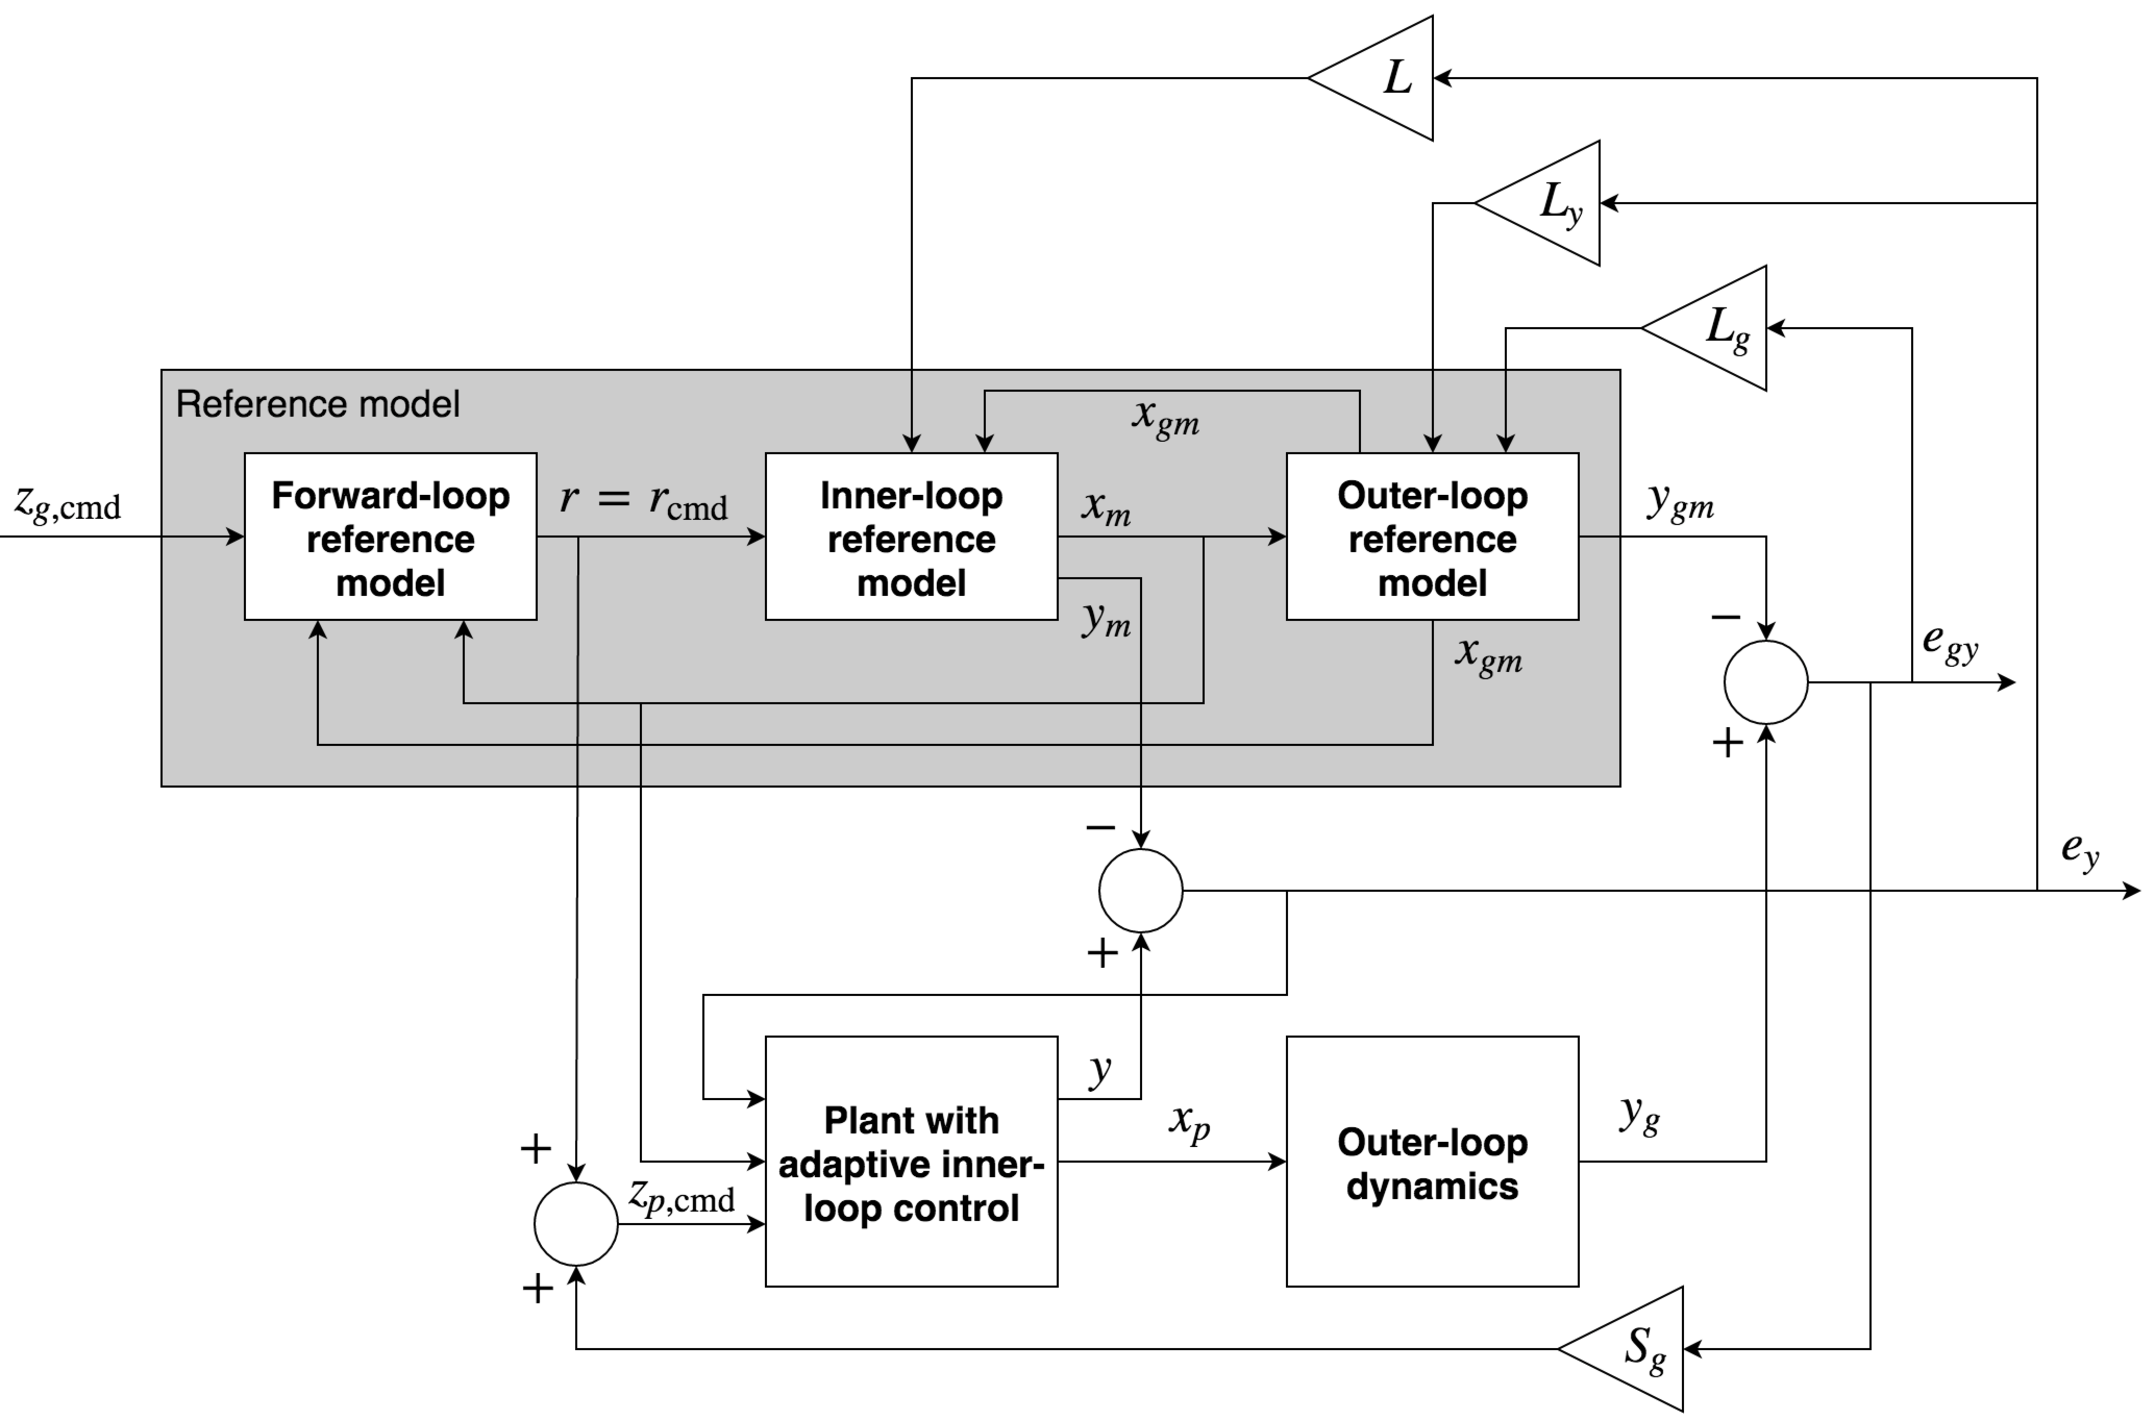
\includegraphics[width=3.0in]{\figurepath/block_adaptive.pdf}
      \vspace{-0.1in}
      \caption{Complete integrated inner and outer-loop design block diagram.\label{fig.innerAndOuterLoopDansOutputFeedback}}
    \end{center}
  \end{figure}

  All that remains to complete the control design is to specify solutions to $L_{y}$, $L_{g}$, and $S_{g}$ such that the closed-loop system is stable and the control goal of command tracking is satisfied.
  The problem is restated as: Find the matrices $L_{y}$, $S_{g}$, $L_{g}$ and $P_{g}$ that together satisfy the following conditions
  \begin{align}
    \label{eqn.theEquation}
    C^{\top}L_{y}^{\top} = - P_{x}B_{\text{cmd}}S_{g}C_{g}P_{g}^{-1} - B_{g}^{\top} & - B_{d}P_{g}^{-1} \\
    \label{eqn.condition3b}
    (A_{g}+L_{g}C_{g})^{\top}P_{g}+P_{g}(A_{g}+L_{g}C_{g}) &< -Q_{g}
  \end{align}
  Rearranging\ \eqref{eqn.theEquation} and using Lemma~\ref{lem.elimination},  the matrices $P_{g}$ and $S_{g}$ must be found satisfying
  {%
    \small
    \begin{align}
      \label{eqn.condition4a}
      -M^{\top}N^{\top}XNB_{\text{cmd}}S_{g}C_{g}P_{g}^{-1} &= M^{\top}(B_{g}^{\top} + B_{d}P_{g}^{-1}) \\
      \label{eqn.condition4b}
      C_{g}^{\top\perp\top} (A_{g}^{\top}P_{g} + P_{g}A_{g}) C_{g}^{\top\perp} &< 0
    \end{align}
  }%
  If $S_{g}$ and $P_{g}$ exist satisfying\ \eqref{eqn.condition4a} and\ \eqref{eqn.condition4b}, then the solution to the outer-loop control problem exists.
  Once solutions $S_{g}$ and $P_{g}$ are found analytically, an $L_{g}$ satisfying\ \eqref{eqn.condition3b} is guaranteed to exist, which can be simply found numerically, as was done to obtain $L$ in the inner-loop design\ \cite{wiese.gnc.2015, wiese.jgcd.2015}.
  With the solutions $S_{g}$ and $P_{g}$, the solution $L_{y}$ from\ \eqref{eqn.theEquation} can then be calculated.
  So the problem that remains is to find $S_{g}$ and $P_{g}$ satisfying\ \eqref{eqn.condition4a} and\ \eqref{eqn.condition4b}.
  The existence of solutions to\ \eqref{eqn.condition4a} is dependent on the sizes of the matrices, as described in the following cases.

  \subsubsection{Case I:\ \texorpdfstring{$n-p=n_{ep}$}{n-p=nep}}

  This case corresponds to the number of inner-loop regulated outputs $n_{ep}$ being equal to the number of unmeasured inner-loop states, given by $n-p$.
  For $S_{g}$ to exist satisfying\ \eqref{eqn.condition4a}, $P_{g}$ must exist satisfying
  \begin{equation}
    \label{eqn.AXBCcase1}
    M^{\top}B_{g}^{\top}P_{g}C_{g}^{\top\perp} = -M^{\top}B_{d}C_{g}^{\top\perp}
  \end{equation}
  with $M^{\top}B_{g}^{\top}\in\mathbb{R}^{n-p\times n_{g}}$ and $C_{g}^{\top\perp}\in\mathbb{R}^{n_{g}\times n_{g}-p_{g}}$.
  $S_{g}$ is then calculated as
  {%
    \small
    \begin{equation}
      \label{eqn.SgCaseI}
      S_{g} = - (M^{\top}N^{\top}XNB_{\text{cmd}})^{-1}M^{\top}(B_{g}^{\top}+B_{d}P_{g}^{-1})P_{g}C_{g}^{-1_{\text{right}}}
    \end{equation}
  }%

  \subsubsection{Case II:\ \texorpdfstring{$n-p<n_{ep}$}{n-p<nep}}

  This case corresponds to the number of inner-loop regulated outputs $n_{ep}$, being greater than the number of unmeasured inner-loop states, given by $n-p$.
  For $S_{g}$ to exist satisfying\ \eqref{eqn.condition4a}, $P_{g}$ must exist satisfying
  \begin{equation}
    \label{eqn.AXBCcase2}
    M^{\top}B_{g}^{\top}P_{g}C_{g}^{\top\perp} = - M^{\top}B_{d}C_{g}^{\top\perp}
  \end{equation}
  Once $P_{g}$ satisfying\ \eqref{eqn.AXBCcase2} is found, $S_{g}$ is determined by
  {%
    \small
    \begin{equation}
      \label{eqn.SgCaseII}
      S_{g} = - (M^{\top}N^{\top}XNB_{\text{cmd}})^{-1_{\text{right}}}M^{\top}(B_{g}^{\top}+B_{d}P_{g}^{-1})P_{g}C_{g}^{-1_{\text{right}}}
    \end{equation}
  }%

  \subsubsection{Case III:\ \texorpdfstring{$n-p>n_{ep}$}{n-p>nep}}

  This case corresponds to the number of inner-loop regulated outputs $n_{ep}$, being less than the number of unmeasured inner-loop states, given by $n-p$.
  In this case $M^{\top}N^{\top}XNB_{\text{cmd}}$ in\ \eqref{eqn.condition4a} is tall, so $S_{g}$ doesn't have the degrees of freedom to satisfy\ \eqref{eqn.condition4a}.

  The conditions for the existence of $S_{g}$ and $P_{g}$ exist satisfying\ \eqref{eqn.condition4a} and\ \eqref{eqn.condition4b} is stated in the following theorem.

  \begin{thm-dan}\label{thm.existenceOuterLoop}
    For the existence of $S_{g}$ and $P_{g}$ satisfying\ \eqref{eqn.condition4a} and\ \eqref{eqn.condition4b} for a stable outer-loop controller, the plant must satisfy $n-p\leq n_{ep}$, $n-p<n_{g}$, the following inequality
    \begin{equation}
      \label{eqn.outerLoopTheoremInequality}
      C_{g}^{\top\perp\top}A_{g}^{\top}(B_{g}M)^{\perp}\bigr(C_{g}^{\top\perp\top}(B_{g}M)^{\perp}\bigr)^{-1_{\textnormal{right}}}
      <
      0
    \end{equation}
    and the rank of the following matrix be full
    \begin{equation*}
      \begin{bmatrix}
        M^{\top}B_{g}^{\top} \\
        C_{g}^{\top\perp}
      \end{bmatrix}
    \end{equation*}
  \end{thm-dan}

  \begin{proof-dan}
    Finding $S_{g}$ and $P_{g}$ satisfying\ \eqref{eqn.condition4a} involves first finding the set of all $P_{g}=P_{g}^{\top}>0$ which satisfy $\Pi_{A}P_{g}\Pi_{B}=\Pi_{C}$, where $\Pi_{A}$, $\Pi_{B}$, and $\Pi_{C}$ are matrices which depend on the state-space plant matrices as in\ \eqref{eqn.AXBCcase1} and\ \eqref{eqn.AXBCcase2}.
    Finding $P_{g}$ involves using a generalized singular value decomposition, and fixes certain elements of $P_{g}$ based on $\Pi_{A}$, $\Pi_{B}$, and $\Pi_{C}$.
    Then, from this set of $P_{g}$, those which also satisfy\ \eqref{eqn.condition4b} are found.
    This involves substituting the form of $P_{g}$ into\ \eqref{eqn.condition4b} and manipulating to obtain\ \eqref{eqn.outerLoopTheoremInequality}.
    These steps are outlined in detail in the following sections.
  \end{proof-dan}

  \begin{rem-dan}
    The control solution is still possible when the inequality in\ \eqref{eqn.outerLoopTheoremInequality} is not strict, which results in\ \eqref{eqn.condition4b} not being strict.
    The implications this has on tracking are discussed following the stability proof, but it is noted that outer-loop command tracking is still achieved as desired.
  \end{rem-dan}

  \begin{rem-dan}
    For the existence of a stable outer loop as described in Theorem~\ref{thm.existenceOuterLoop} for the case when $n-p\geq n_{g}$, a solution is still possible, but requires additional constraints to be satisfied.
  \end{rem-dan}

  \section{Solving \texorpdfstring{$P_{g}$}{Pg}: Symmetric Solutions to the Matrix Equation \texorpdfstring{$\Pi_{A}P_{g}\Pi_{B}=\Pi_{C}$}{piAPgpiB=piC}}

  Equations\ \eqref{eqn.AXBCcase1} and\ \eqref{eqn.AXBCcase2} are in the form $\Pi_{A}P_{g}\Pi_{B}=\Pi_{C}$.
  In these two cases, the matrices $\Pi_{A}$, $\Pi_{B}$, and $\Pi_{C}$ in\ \eqref{eqn.AXBCcase1} and\ \eqref{eqn.AXBCcase2} are given by
  \begin{equation}
    \label{eqn.AXBandCCaseI}
    \begin{split}
      \Pi_{A} &= M^{\top}B_{g}^{\top} \\
      \Pi_{B} &= C_{g}^{\top\perp} \\
      \Pi_{C} &= -M^{\top}B_{d}C_{g}^{\top\perp} \\
    \end{split}
  \end{equation}
  where $\Pi_{A}\in\mathbb{R}^{n-p\times n_{g}}$, $P_{g}\in\mathbb{R}^{n_{g}\times n_{g}}$, $\Pi_{B}\in\mathbb{R}^{n_{g}\times n_{g}-p_{g}}$ and $\Pi_{C}\in\mathbb{R}^{n-p\times n_{g}-p_{g}}$.
  Using the definitions in\ \eqref{eqn.AXBandCCaseI}, the inequality\ \eqref{eqn.condition4b} is rewritten and the problem once again restated as: Find $P_{g}=P_{g}^{\top}>0$ satisfying
  \begin{align}
    \label{eqn.PiAPgPiBPiC}
    \Pi_{A}P_{g}\Pi_{B} &= \Pi_{C} \\
    \label{eqn.condition4bCaseI}
    \Pi_{B}^{\top} (A_{g}^{\top}P_{g} + P_{g}A_{g}) \Pi_{B} &< 0
  \end{align}

  \subsection{A Generalized Singular Value Decomposition}

  Determining solutions $P_{g}$ to Eq.\ \eqref{eqn.PiAPgPiBPiC} involves first decomposing $\Pi_{A}$ and $\Pi_{B}$ using a generalized singular value decomposition (GSVD)\ \cite{golub.matrix.1996,dai.symmetric.1996,paige.towardsgsvd.1981,hua.symmetric.1990} as follows
  \begin{equation}
    \label{eqn.AandBGSVD}
    \begin{split}
      \Pi_{A} &= U\Sigma_{A}P \\
      \Pi_{B}^{\top} &= V\Sigma_{B}P
    \end{split}
  \end{equation}
  where $U\in\mathbb{R}^{n-p\times n-p}$ and $V\in\mathbb{R}^{n_{g}-p_{g}\times n_{g}-p_{g}}$, $P\in\mathbb{R}^{n_{g}\times n_{g}}$, and $\Sigma_{A}\in\mathbb{R}^{n-p\times n_{g}}$ and $\Sigma_{B}\in\mathbb{R}^{n_{g}-p_{g}\times n_{g}}$.
  The matrices describing the decomposition in Eq.\ \eqref{eqn.AandBGSVD} are given by
  {%
    \small
    \begin{equation}
      \label{eqn.SigmaASigmaB}
      \begin{split}
        \Sigma_{A}
        &=
        \begin{bmatrix}
          I_{n-p\times n-p} & 0_{n-p\times n_{g}-p_{g}} & 0_{n-p\times p-n+p_{g}}
        \end{bmatrix} \\
        \Sigma_{B}
        &=
        \begin{bmatrix}
          0_{n_{g}-p_{g}\times n-p} & I_{n_{g}-p_{g}\times n_{g}-p_{g}} & 0_{n_{g}-p_{g}\times p-n+p_{g}}
        \end{bmatrix} \\
      \end{split}
    \end{equation}
  }%
  and
  \begin{equation}
    \label{eqn.P}
    P = P_{\Lambda}
    \begin{bmatrix}
      \Pi_{A} \\
      \Pi_{B}^{\top} \\
      \begin{bmatrix}
        \Pi_{A}^{\top} & \Pi_{B}
      \end{bmatrix}^{\perp\top} \\
    \end{bmatrix}
  \end{equation}
  where $P_{\Lambda}$ is an arbitrary block diagonal matrix, with full rank, given by
  \begin{equation}
    \label{eqn.PLambda}
    P_{\Lambda} =
    \begin{bmatrix}
      P_{A} & 0 & 0 \\
      0 & P_{B} & 0 \\
      0 & 0 & P_{N}
    \end{bmatrix}
  \end{equation}
  where $P_{A}\in\mathbb{R}^{n-p\times n-p}$, $P_{B}\in\mathbb{R}^{n_{g}-p_{g}\times n_{g}-p_{g}}$, and $P_{N}\in\mathbb{R}^{p+p_{g}-n \times p+p_{g}-n}$ are each matrices of full rank.
  Substituting\ \eqref{eqn.PLambda} into\ \eqref{eqn.P} gives
  \begin{equation}
    \label{eqn.PP}
    P
    =
    \begin{bmatrix}
      P_{A}\Pi_{A} \\
      P_{B}\Pi_{B}^{\top} \\
      P_{N}
      \begin{bmatrix}
        \Pi_{A}^{\top} & \Pi_{B}
      \end{bmatrix}^{\perp\top} \\
    \end{bmatrix}
  \end{equation}
  Selecting $U$ and $V$ in\ \eqref{eqn.AandBGSVD} as $U=P_{A}^{-1}$ and $V=P_{B}^{-1}$ ensures that the decomposition\ \eqref{eqn.AandBGSVD} holds.

  \subsection{Satisfying \texorpdfstring{$\Pi_{A}P_{g}\Pi_{B}=\Pi_{C}$}{piAPgpiB=piC} with \texorpdfstring{$P_{g}=P_{g}^{\top}>0$}{Pg=PgT}}

  Substituting $\Pi_{A}$ and $\Pi_{B}$ decomposed as in\ \eqref{eqn.AandBGSVD} into\ \eqref{eqn.PiAPgPiBPiC} gives
  \begin{equation}
    \label{eqn.USigmaAPXPSigmaBVC}
    U\Sigma_{A}PP_{g}P^{\top}\Sigma_{B}^{\top}V^{\top} = \Pi_{C}
  \end{equation}
  Propose the following solution $P_{g}$ to\ \eqref{eqn.USigmaAPXPSigmaBVC}
  \begin{equation}
    \label{eqn.Pg}
    P_{g} = P^{-1}X_{D}P^{-\top}
  \end{equation}
  where $X_{D}=X_{D}^{\top}>0$ ensures that $P_{g}=P_{g}^{\top}>0$.
  Substituting $P_{g}$ from\ \eqref{eqn.Pg} into\ \eqref{eqn.USigmaAPXPSigmaBVC} results in
  \begin{equation*}
    U\Sigma_{A}PP^{-1}X_{D}P^{-\top} P^{\top}\Sigma_{B}^{\top}V^{\top}
    =
    \Pi_{C}
  \end{equation*}
  which can be simplified as
  \begin{equation}
    \label{eqn.USigmaAXDSigmaBV}
    U\Sigma_{A}X_{D}\Sigma_{B}^{\top}V^{\top} = \Pi_{C}
  \end{equation}
  The matrix $X_{D}=X_{D}^{\top}>0$ is written as
  \begin{equation}
    \label{eqn.XD}
    X_{D} =
    \begin{bmatrix}
      X_{D11} & X_{D12} & X_{D13} \\
      X_{D12}^{\top} & X_{D22} & X_{D23} \\
      X_{D13}^{\top} & X_{D23}^{\top} & X_{D33} \\
    \end{bmatrix}
  \end{equation}
  where $X_{D11}\in\mathbb{R}^{n-p\times n-p}$, $X_{D12}\in\mathbb{R}^{n-p\times n_{g}-p_{g}}$, $X_{D13}\in\mathbb{R}^{n-p\times p-n+p_{g}}$, $X_{D22}\in\mathbb{R}^{n_{g}-p_{g}\times n_{g}-p_{g}}$, $X_{D23}\in\mathbb{R}^{n_{g}-p_{g}\times p-n+p_{g}}$, and $X_{D33}\in\mathbb{R}^{p-n+p_{g}\times p-n+p_{g}}$.
  Substituting the form of $X_{D}$ from\ \eqref{eqn.XD} and $\Sigma_{A}$ and $\Sigma_{B}$ from\ \eqref{eqn.SigmaASigmaB} into\ \eqref{eqn.USigmaAXDSigmaBV} gives
  \begin{equation*}
    U
    \begin{bmatrix}
      I & 0 & 0
    \end{bmatrix}
    \begin{bmatrix}
      X_{D11} & X_{D12} & X_{D13} \\
      X_{D12}^{\top} & X_{D22} & X_{D23} \\
      X_{D13}^{\top} & X_{D23}^{\top} & X_{D33} \\
    \end{bmatrix}
    \begin{bmatrix}
      0 \\
      I \\
      0
    \end{bmatrix}
    V^{\top}
    = \Pi_{C}
  \end{equation*}
  from which $X_{D12}$ is given as
  \begin{equation}
    \label{eqn.XD12}
    X_{D12} = P_{A}\Pi_{C}P_{B}^{\top}
  \end{equation}
  The choice of $X_{D12}$ in\ \eqref{eqn.XD12} ensures that $P_{g}$ given by\ \eqref{eqn.Pg} with $X_{D}$ given by\ \eqref{eqn.XD} satisfies the equation $\Pi_{A}P_{g}\Pi_{B}=\Pi_{C}$.
  However, the remaining degrees of freedom in $X_{D}$ must be selected to ensure also that $P_{g}>0$, and that $P_{g}$ also satisfies the inequality\ \eqref{eqn.condition4bCaseI}.

  \subsection{Satisfying \texorpdfstring{$\Pi_{B}^{\top} (A_{g}^{\top}P_{g} + P_{g}A_{g}) \Pi_{B} < 0$}{}}

  With $P_{g}$ given by\ \eqref{eqn.Pg} dependent on $X_{D}$ given in\ \eqref{eqn.XD} with $X_{D12}$ given in\ \eqref{eqn.XD12} and $P$ given in\ \eqref{eqn.PP}, the goal now is to find the remaining elements of $X_{D}$ so that the resulting $P_{g}$ satisfies the inequality\ \eqref{eqn.condition4bCaseI} and ensures $P_{g}>0$.
  Substituting $P_{g}$ from\ \eqref{eqn.Pg} into\ \eqref{eqn.condition4bCaseI} gives
  {%
    \small
    \begin{equation}
      \label{eqn.condition4bCaseI3}
      \Pi_{B}^{\top}P^{-1} (PA_{g}^{\top}P^{-1}X_{D} + X_{D}P^{-\top}A_{g}P^{\top}) P^{-\top}\Pi_{B} < 0
    \end{equation}
  }%
  Given $P$ in\ \eqref{eqn.P} its inverse $P^{-1}$ must satisfy
  \begin{equation}
    \label{eqn.PexpandedTimesPinv}
    \begin{bmatrix}
      P_{A}\Pi_{A} \\
      P_{B}\Pi_{B}^{\top} \\
      P_{N}
      \begin{bmatrix}
        \Pi_{A}^{\top} & \Pi_{B}
      \end{bmatrix}^{\perp\top} \\
    \end{bmatrix}
    P^{-1}
    =
    \begin{bmatrix}
      I & 0 & 0 \\
      0 & I & 0 \\
      0 & 0 & I \\
    \end{bmatrix}
  \end{equation}
  It can be seen from this that
  \begin{equation}
    \label{eqn.BTPinv}
    \Pi_{B}^{\top}P^{-1} =
    \begin{bmatrix}
      0 & P_{B}^{-1} & 0
    \end{bmatrix}
  \end{equation}
  Using\ \eqref{eqn.BTPinv}, the inequality\ \eqref{eqn.condition4bCaseI3} becomes
  {%
    \small
    \begin{equation}
      \label{eqn.condition4bCaseI4}
      \begin{bmatrix}
        0 & P_{B}^{-1} & 0
      \end{bmatrix}
      (PA_{g}^{\top}P^{-1}X_{D} + X_{D}P^{-\top}A_{g}P^{\top})
      \begin{bmatrix}
        0 \\
        P_{B}^{-\top} \\
        0 \\
      \end{bmatrix}
      < 0
    \end{equation}
  }%
  Defining $\bar{P}$ as
  \begin{equation}
    \label{eqn.Pbar}
    \bar{P} = PA_{g}^{\top}P^{-1}
  \end{equation}
  the inequality\ \eqref{eqn.condition4bCaseI4} can be written as
  \begin{equation}
    \label{eqn.condition4bCaseI5}
    \begin{bmatrix}
      0 & P_{B}^{-1} & 0
    \end{bmatrix}
    (\bar{P}X_{D} + X_{D}\bar{P}^{\top})
    \begin{bmatrix}
      0 \\
      P_{B}^{-\top} \\
      0 \\
    \end{bmatrix}
    < 0
  \end{equation}
  Examining\ \eqref{eqn.PexpandedTimesPinv} it can be seen that the columns of $P^{-1}$ are given by
  {%
    \small
    \begin{equation}
      \label{eqn.PPinv}
      P^{-1} =
      \begin{bmatrix}
        \Pi_{B}^{\perp}\bigr(P_{A}\Pi_{A}\Pi_{B}^{\perp}\bigr)^{-1_{\text{right}}}
        &
        \Pi_{A}^{\top\perp}\bigr(P_{B}\Pi_{B}^{\top}\Pi_{A}^{\top\perp}\bigr)^{-1_{\text{right}}}
        &
        \times
      \end{bmatrix}
    \end{equation}
  }%
  where $\times$ indicates a column of $P^{-1}$ which is to remain unspecified.
  Expanding $P$ and $P^{-1}$, the requirement that $PP^{-1}=I$ requires the following conditions be satisfied
  \begin{equation}
    \label{eqn.firstColumnOfPinv}
    \begin{split}
      P_{A}\Pi_{A}\Pi_{B}^{\perp}\bigr(P_{A}\Pi_{A}\Pi_{B}^{\perp}\bigr)^{-1_{\text{right}}} &= I \\
      P_{B}\Pi_{B}^{\top}\Pi_{B}^{\perp}\bigr(P_{A}\Pi_{A}\Pi_{B}^{\perp}\bigr)^{-1_{\text{right}}} &= 0 \\
      P_{N}
      \begin{bmatrix}
        \Pi_{A}^{\top} & \Pi_{B}
      \end{bmatrix}^{\perp\top}
      \Pi_{B}^{\perp}\bigr(P_{A}\Pi_{A}\Pi_{B}^{\perp}\bigr)^{-1_{\text{right}}} &= 0
    \end{split}
  \end{equation}
  and
  \begin{equation}
  \label{eqn.secondColumnOfPinv}
    \begin{split}
      P_{A}\Pi_{A}\Pi_{A}^{\top\perp}\bigr(P_{B}\Pi_{B}^{\top}\Pi_{A}^{\top\perp}\bigr)^{-1_{\text{right}}}
      &= 0 \\
      P_{B}\Pi_{B}^{\top}\Pi_{A}^{\top\perp}\bigr(P_{B}\Pi_{B}^{\top}\Pi_{A}^{\top\perp}\bigr)^{-1_{\text{right}}}
      &= I \\
      P_{N}
      \begin{bmatrix}
        \Pi_{A}^{\top} & \Pi_{B}
      \end{bmatrix}^{\perp\top}
      \Pi_{A}^{\top\perp}\bigr(P_{B}\Pi_{B}^{\top}\Pi_{A}^{\top\perp}\bigr)^{-1_{\text{right}}}
      &= 0 \\
    \end{split}
  \end{equation}
  The first two conditions in\ \eqref{eqn.firstColumnOfPinv} and\ \eqref{eqn.secondColumnOfPinv} are obvious, following from the definition of the right inverse, and properties of the annihilator matrices.
  With $P^{-1}$ given by\ \eqref{eqn.PPinv}, $\bar{P}$ in\ \eqref{eqn.Pbar} can be written as
  {%
    \small
    \begin{equation}
      \label{eqn.Pbar2}
      \bar{P} =
      \begin{bmatrix}
        P_{A}\Pi_{A} \\
        P_{B}\Pi_{B}^{\top} \\
        P_{N}
        \begin{bmatrix}
          \Pi_{A}^{\top} & \Pi_{B}
        \end{bmatrix}^{\perp\top} \\
      \end{bmatrix}
      A_{g}^{\top}
      \begin{bmatrix}
        (\Pi_{B}^{\perp}\bigr(P_{A}\Pi_{A}\Pi_{B}^{\perp}\bigr)^{-1_{\text{right}}})^{\top} \\
        (\Pi_{A}^{\top\perp}\bigr(P_{B}\Pi_{B}^{\top}\Pi_{A}^{\top\perp}\bigr)^{-1_{\text{right}}})^{\top} \\
        \times
      \end{bmatrix}^{\top}
    \end{equation}
  }%
  where $\times$ in\ \eqref{eqn.Pbar2} again represents an element of $\bar{P}$ which remains unspecified.
  $\bar{P}$ can also be partitioned into a block matrix given by
  \begin{equation}
    \label{eqn.PbarPartitioned}
    \bar{P} =
    \begin{bmatrix}
      \bar{P}_{11} & \bar{P}_{12} & \bar{P}_{13} \\
      \bar{P}_{21} & \bar{P}_{22} & \bar{P}_{23}\\
      \bar{P}_{31} & \bar{P}_{32} & \bar{P}_{33}\\
    \end{bmatrix}
  \end{equation}
  where $P_{11}\in\mathbb{R}^{n-p \times n-p}$, $P_{12}\in\mathbb{R}^{n-p \times n_{g}-p_{g}}$, $P_{13}\in\mathbb{R}^{n-p \times p-n+p_{g}}$, $P_{21}\in\mathbb{R}^{n_{g}-p_{g} \times n-p}$, $P_{22}\in\mathbb{R}^{n_{g}-p_{g} \times n_{g}-p{g}}$, $P_{23}\in\mathbb{R}^{n_{g}-p_{g} \times p-n+p_{g}}$, $P_{31}\in\mathbb{R}^{p-n+p_{g} \times n-p}$, $P_{32}\in\mathbb{R}^{p-n+p_{g} \times n_{g}-p_{g}}$, and $P_{33}\in\mathbb{R}^{p-n+p_{g} \times p-n+p_{g}}$ with $\bar{P}_{21}$ and $\bar{P}_{22}$ given by
  \begin{equation}
    \label{eqn.Pbar21andPbar22}
    \begin{split}
      \bar{P}_{21}
      &=
      P_{B}\Pi_{B}^{\top}A_{g}^{\top}\Pi_{B}^{\perp}
      \bigr(P_{A}\Pi_{A}\Pi_{B}^{\perp}\bigr)^{-1_{\text{right}}} \\
      \bar{P}_{22}
      &=
      P_{B}\Pi_{B}^{\top}A_{g}^{\top}\Pi_{A}^{\top\perp}\bigr(P_{B}\Pi_{B}^{\top}\Pi_{A}^{\top\perp}\bigr)^{-1_{\text{right}}}
    \end{split}
  \end{equation}
  The inequality in\ \eqref{eqn.condition4bCaseI5} with $\bar{P}$ given by\ \eqref{eqn.PbarPartitioned}, where $\bar{P}_{21}$ and $\bar{P}_{22}$ are given by\ \eqref{eqn.Pbar21andPbar22}, and $X_{D}$ given by\ \eqref{eqn.XD} must be satisfied by the selection of the remaining elements of $X_{D}$.
  Plugging these expressions for $\bar{P}$ in\ \eqref{eqn.PbarPartitioned} and $X_{D}$ in\ \eqref{eqn.XD} into the inequality in\ \eqref{eqn.condition4bCaseI5} gives
  {%
    \small
    \begin{equation*}
      \begin{split}
        &
        \begin{bmatrix}
          0 \\
          P_{B}^{-\top} \\
          0
        \end{bmatrix}^{\top}
        \left(
        \begin{bmatrix}
          \bar{P}_{11} & \bar{P}_{12} & \bar{P}_{13} \\
          \bar{P}_{21} & \bar{P}_{22} & \bar{P}_{23}\\
          \bar{P}_{31} & \bar{P}_{32} & \bar{P}_{33}\\
        \end{bmatrix}
        \right.
        \begin{bmatrix}
          X_{D11} & X_{D12} & X_{D13} \\
          X_{D12}^{\top} & X_{D22} & X_{D23} \\
          X_{D13}^{\top} & X_{D23}^{\top} & X_{D33} \\
        \end{bmatrix} \\
        &+
        \begin{bmatrix}
          X_{D11} & X_{D12} & X_{D13} \\
          X_{D12}^{\top} & X_{D22} & X_{D23} \\
          X_{D13}^{\top} & X_{D23}^{\top} & X_{D33} \\
        \end{bmatrix}
        \left.
        \begin{bmatrix}
          \bar{P}_{11}^{\top} & \bar{P}_{21}^{\top} & \bar{P}_{31}^{\top} \\
          \bar{P}_{12}^{\top} & \bar{P}_{22}^{\top} & \bar{P}_{32}^{\top}\\
          \bar{P}_{13}^{\top} & \bar{P}_{23}^{\top} & \bar{P}_{33}^{\top}\\
        \end{bmatrix}
        \right)
        \begin{bmatrix}
          0 \\
          P_{B}^{-\top} \\
          0 \\
        \end{bmatrix}
        < 0
      \end{split}
    \end{equation*}
  }%
  which is equivalent to
  \begin{equation}
    \label{eqn.condition4bCaseI7}
    \begin{split}
      &\bar{P}_{21}X_{D12} + \bar{P}_{22}X_{D22} + \bar{P}_{23}X_{D23}^{\top} \\
      & \quad + X_{D12}^{\top}\bar{P}_{21}^{\top} + X_{D22}\bar{P}_{22}^{\top} + X_{D23}^{\top}\bar{P}_{23}^{\top}
      < 0
    \end{split}
  \end{equation}
  $X_{D12}$ in\ \eqref{eqn.condition4bCaseI7} is given by\ \eqref{eqn.XD12} thus ensuring $\Pi_{A}P_{g}\Pi_{B}=\Pi_{C}$.
  The remaining elements of $X_{D}$ must be selected so that $X_{D}>0$ and so as to satisfy the inequality in Eq.\ \eqref{eqn.condition4bCaseI7}.
  Rearranging the terms in\ \eqref{eqn.condition4bCaseI7} gives
  {%
    \small
    \begin{equation}
      \label{eqn.condition4bCaseI8}
      \begin{split}
        &(\bar{P}_{22}X_{D22} + X_{D22}\bar{P}_{22}^{\top})
        +(\bar{P}_{21}X_{D12} + X_{D12}^{\top}\bar{P}_{21}^{\top}) \\
        & \quad <
        -(\bar{P}_{23}X_{D23}^{\top} + X_{D23}^{\top}\bar{P}_{23}^{\top})
      \end{split}
    \end{equation}
  }%
  The problem now is to select the remaining elements of $X_{D}$ so as to satisfy\ \eqref{eqn.condition4bCaseI8}, while also ensuring $X_{D}>0$.

  \subsection{Solving for \texorpdfstring{$X_{D}$}{XD}}

  To satisfy\ \eqref{eqn.condition4bCaseI8} and ensure $X_{D}>0$ in\ \eqref{eqn.XD}, the solution $X_{D12}$ from\ \eqref{eqn.XD12} is used, and setting $X_{D13} = 0$, $X_{D23} = 0$, and $X_{D33} > 0$ simplifies\ \eqref{eqn.condition4bCaseI8} to
  {%
    \small
    \begin{equation}
      \label{eqn.condition4bCaseI9}
      (\bar{P}_{22}X_{D22} + X_{D22}\bar{P}_{22}^{\top})
      +(\bar{P}_{21}X_{D12} + X_{D12}^{\top}\bar{P}_{21}^{\top})
      <
      0
    \end{equation}
  }%
  and $X_{D}$ in\ \eqref{eqn.XD} to
  \begin{equation}
    \label{eqn.XDblock}
    X_{D} =
    \begin{bmatrix}
      X_{D11} & X_{D12} & 0 \\
      X_{D12}^{\top} & X_{D22} & 0 \\
      0 & 0 & X_{D33} \\
    \end{bmatrix}
  \end{equation}
  If $\bar{P}_{22}$ in\ \eqref{eqn.condition4bCaseI9} is stable, this Lyapunov equation\ \eqref{eqn.condition4bCaseI9} can be solved to obtain $X_{D22}$.
  Then with $X_{D12}$, $X_{D22}$, and $X_{D33}$ fixed, the Schur Complement is then used to selected $X_{D11}$ to ensure $X_{D}>0$ in\ \eqref{eqn.XDblock}.
  With $\bar{P}_{22}$ given by\ \eqref{eqn.Pbar21andPbar22}, this provides an easy way to check if the outer-loop control solution exists.
  However, if $\bar{P}_{22}$ in\ \eqref{eqn.condition4bCaseI9} is not stable, this inequality may still be satisfied, based on the properties of $\bar{P}_{21}$ and $X_{D12}$.
  Thus, in this case, these properties must be examined to determine whether the outer-loop control solution exists.
  These two cases are considered in the following subsections.

  \subsubsection{Case i: \texorpdfstring{$\bar{P}_{22}$}{P22} is Stable}

  If $\bar{P}_{22}$ in\ \eqref{eqn.condition4bCaseI9} is stable, this Lyapunov equation can be solved to obtain $X_{D22}$.
  Then, $X_{D11}>0$ can be selected satisfying the following Schur complement
  \begin{equation}
    \label{eqn.XD11}
    X_{D11} > X_{D12}X_{D22}^{-1}X_{D12}^{\top}
  \end{equation}
  which ensures that $P_{g}$ satisfies $\Pi_{A}P_{g}\Pi_{B}=\Pi_{C}$ with $P_{g}=P_{g}^{\top}>0$, and also satisfies the inequality\ \eqref{eqn.condition4bCaseI}.
  Thus, satisfaction of the inequality\ \eqref{eqn.condition4bCaseI} and existence of the outer-loop controller is dependent on $\bar{P}_{22}$ in\ \eqref{eqn.Pbar21andPbar22} being stable.
  Stability of $\bar{P}_{22}$ in\ \eqref{eqn.Pbar21andPbar22} is equivalent to the following
  \begin{equation}
    \label{eqn.CaseITheoremInequality}
    \Pi_{B}^{\top}A_{g}^{\top}\Pi_{A}^{\top\perp}\bigr(\Pi_{B}^{\top}\Pi_{A}^{\top\perp}\bigr)^{-1_{\text{right}}} < 0
  \end{equation}
  Using the notation in\ \eqref{eqn.AXBandCCaseI}, the requirement in\ \eqref{eqn.CaseITheoremInequality} can be written as
 \ \eqref{eqn.outerLoopTheoremInequality}.
  If\ \eqref{eqn.outerLoopTheoremInequality} is satisfied, then $X_{D}=X_{D}^{\top}>0$ exists which defines $P_{g}$ and ensures that $P_{g}=P_{g}^{\top}>0$, $\Pi_{A}P_{g}\Pi_{B}=\Pi_{C}$ as in\ \eqref{eqn.PiAPgPiBPiC}, and $\Pi_{B}^{\top}(A_{g}^{\top}P_{g}+P_{g}A_{g})\Pi_{B}<0$ as in\ \eqref{eqn.condition4bCaseI}.

  \subsubsection{Case ii: \texorpdfstring{$\bar{P}_{22}$}{P22} is Not Stable}

  If $\bar{P}_{22}$ is not stable, the inequality\ \eqref{eqn.condition4bCaseI9} can still be satisfied if
  \begin{equation}
    \label{eqn.SecondLyapunovEquation}
    (\bar{P}_{21}X_{D12} + X_{D12}^{\top}\bar{P}_{21}^{\top}) < 0
  \end{equation}
  In this case, $X_{D22}$ can be selected sufficiently small so that the negative term\ \eqref{eqn.SecondLyapunovEquation} in\ \eqref{eqn.condition4bCaseI9} ensures the inequality is satisfied.
  Using the expressions for $\bar{P}_{12}$ from\ \eqref{eqn.Pbar21andPbar22} and $X_{D12}$ from\ \eqref{eqn.XD12} to evaluate the quantity $\bar{P}_{21}X_{D12}$ in\ \eqref{eqn.SecondLyapunovEquation} gives
  {%
    \small
    \begin{equation}
      \label{eqn.Pbar21XD12}
      \bar{P}_{21}X_{D12}
      =
      P_{B}\Pi_{B}^{\top}A_{g}^{\top}\Pi_{B}^{\perp}
      \bigr(P_{A}\Pi_{A}\Pi_{B}^{\perp}\bigr)^{-1_{\text{right}}}
      P_{A}\Pi_{C}P_{B}^{\top}
    \end{equation}
  }%
  The matrix $\bar{P}_{21}X_{D12}$ in\ \eqref{eqn.Pbar21XD12} is square, with dimensions $n_{g}-p_{g}\times n_{g}-p_{g}$.
  Using the expression for $\bar{P}_{21}X_{D12}$ in\ \eqref{eqn.Pbar21XD12} allows the inequality in\ \eqref{eqn.SecondLyapunovEquation} to be expressed as
  {%
    \small
    \begin{equation}
      \label{eqn.Pbar21XD12lyapInequality}
      \begin{split}
        &
        P_{B}\Pi_{B}^{\top}A_{g}^{\top}\Pi_{B}^{\perp}
        \bigr(P_{A}\Pi_{A}\Pi_{B}^{\perp}\bigr)^{-1_{\text{right}}}
        P_{A}\Pi_{C}P_{B}^{\top}  \\
        & +
        \bigr(
        P_{B}\Pi_{B}^{\top}A_{g}^{\top}\Pi_{B}^{\perp}
        \bigr(P_{A}\Pi_{A}\Pi_{B}^{\perp}\bigr)^{-1_{\text{right}}}
        P_{A}\Pi_{C}P_{B}^{\top}
        \bigr)^{\top}
        <0
      \end{split}
    \end{equation}
  }%
  Satisfying the inequality in\ \eqref{eqn.Pbar21XD12lyapInequality} is independent of the selection of the matrices $P_{A}$ and $P_{B}$.
  Thus, satisfying the inequality in\ \eqref{eqn.Pbar21XD12lyapInequality} is equivalent to satisfying
  \begin{equation}
    \label{eqn.Pbar21XD12lyapInequality3}
    \begin{split}
      &
      \Pi_{B}^{\top}A_{g}^{\top}\Pi_{B}^{\perp}
      \bigr(\Pi_{A}\Pi_{B}^{\perp}\bigr)^{-1_{\text{right}}}
      \Pi_{C}  \\
      +
      \bigr(
      &
      \Pi_{B}^{\top}A_{g}^{\top}\Pi_{B}^{\perp}
      \bigr(\Pi_{A}\Pi_{B}^{\perp}\bigr)^{-1_{\text{right}}}
      \Pi_{C}
      \bigr)^{\top}
      <0
    \end{split}
  \end{equation}
  Plugging in expressions for $\Pi_{A}$, $\Pi_{B}$ and $\Pi_{C}$ from\ \eqref{eqn.AXBandCCaseI} in terms of the plant state-space matrices into\ \eqref{eqn.Pbar21XD12lyapInequality3} gives
  {%
    \small
    \begin{equation}
      \label{eqn.otherConditionForStability}
      \begin{split}
        &-(C_{g}^{\top\perp\top}A_{g}^{\top}C_{g}^{\top}C_{g}B_{g}MM^{\top}B_{d}C_{g}^{\top\perp}) \\
        & \quad -
        (C_{g}^{\top\perp\top}A_{g}^{\top}C_{g}^{\top}C_{g}B_{g}MM^{\top}B_{d}C_{g}^{\top\perp})^{\top}
        <0
      \end{split}
    \end{equation}
  }%
  Thus, when $\bar{P}_{22}$ in\ \eqref{eqn.condition4bCaseI9} is not stable, a solution still exists if\ \eqref{eqn.otherConditionForStability} is satisfied.
  In this case, $X_{D22}$ can be selected sufficiently small so that the negative term\ \eqref{eqn.SecondLyapunovEquation} in\ \eqref{eqn.condition4bCaseI9} ensures the inequality is satisfied.
  Thus in this case even if\ \eqref{eqn.outerLoopTheoremInequality} in Theorem~\ref{thm.existenceOuterLoop} does not hold, a control solution still exists if\ \eqref{eqn.otherConditionForStability} is satisfied.

  \subsection{Degrees of Freedom}

  The degrees of freedom available to the control designer are the matrices $P_{A}$, $P_{B}$, and $P_{N}$ in $P_{\Lambda}$ and thus $P$ as in\ \eqref{eqn.PP}, that can be selected arbitrarily as long as they are full rank.
  In addition $X_{D}>0$ contains several degrees of freedom.
  The matrix $X_{D33}=X_{D33}^{\top}>0$ is arbitrary, $X_{D22}$ can be selected as desired satisfying\ \eqref{eqn.condition4bCaseI9}, and finally $X_{D11}$ can be selected using the Schur complement to ensure $X_{D}>0$.

  \section{Solving for Remaining Outer-Loop Controller Gains}

  With the solution $P_{g}$ determined, $S_{g}$ can now be determined from\ \eqref{eqn.SgCaseI} or\ \eqref{eqn.SgCaseII}, depending on the dimensions.
  With this $P_{g}$, an $L_{g}$ satisfying the inequality in\ \eqref{eqn.condition4a} is guaranteed to exist and can be solved for numerically.
  The CRM gain $L_{y}$ can then be solved from\ \eqref{eqn.theEquation} as
  {%
    \small
    \begin{equation}
      \label{eqn.Ly}
      L_{y}
      =
      -\bigr((P_{x}B_{\text{cmd}}S_{g}C_{g}P_{g}^{-1})^{\top} + B_{g} + P_{g}^{-\top}B_{d}^{\top}\bigr)C^{-1_{\text{right}}}
    \end{equation}
  }%
  The matrix $L_{y}$ modifies the outer-loop guidance portion of the reference model in response to errors within the inner loop.
  It is this feature which enables stability of the combined inner and outer loops, and provides command tracking at the outer loop.
  The stability of the complete system using the adaptive inner-loop and sequential loop closure procedure to close the outer loop is given in Theorem~\ref{thm.outerloop}.

  \begin{rem-dan}
    When the outer-loop kinematics do not affect the inner-loop dynamics at all, that is when $B_{d}=0$, then $P_{g}$ changes the solution to $S_{g}$ as given by\ \eqref{eqn.SgCaseI} and\ \eqref{eqn.SgCaseII}, but has no effect on $L_{y}$.
    This can see this by plugging in the solution $S_{g}$ from\ \eqref{eqn.SgCaseI} or\ \eqref{eqn.SgCaseII} into\ \eqref{eqn.Ly}, resulting in $P_{g}$ canceling out.
    This is important to note when tuning the outer-loop controller.
  \end{rem-dan}


  \section{Stability}

  The inner-loop error dynamics were given in\ \eqref{eqn.errordynamics1} and a Lyapunov function provided in\ \eqref{eqn.lyapfunction}, which showed stability of the closed loop system with update law in\ \eqref{eqn.updatelaw}.
  When the outer-loop dynamics were considered, the assumption that $B_{d}=0$ when designing the inner-loop controller was relaxed, giving the modified inner-loop dynamics in\ \eqref{eqn.uncsystemWithBd}.
  This change to the inner-loop plant dynamics modified the inner-loop error dynamics in\ \eqref{eqn.errordynamics1} to those in\ \eqref{eqn.errordynamics4}.
  The inner and outer-loop error dynamics in\ \eqref{eqn.innerAndOuterLoopErrorDynamics1} can be written in matrix form as
  {%
    \small
    \begin{equation}
      \label{eqn.innerAndOuterLoopErrorDynamics2}
      \begin{split}
        &
        \begin{bmatrix}
          \dot{e}_{x}(t) \\
          \dot{e}_{g}(t)
        \end{bmatrix}
        =
        \begin{bmatrix}
          A+LC+B\Psi^{\top} & B_{\text{cmd}}S_{g}C_{g} + B_{d} \\
          B_{g}+L_{y}C & A_{g}+L_{g}C_{g}
        \end{bmatrix}
        \begin{bmatrix}
          e_{x}(t) \\
          e_{g}(t)
        \end{bmatrix} \\
        & +
        \begin{bmatrix}
          B \\
          0
        \end{bmatrix}
        \Lambda\widetilde{\Theta}^{\top}(t)x_{m}(t)
      \end{split}
    \end{equation}
  }%
  The stability of the closed-loop system with the error dynamics in\ \eqref{eqn.innerAndOuterLoopErrorDynamics2} is proved in the following theorem.

  \begin{thm-dan}\label{thm.outerloop}
    The uncertain system in\ \eqref{eqn.wholeSystemUncertain} with inner-loop controller specified by the control law in\ \eqref{eqn.u}, update law in\ \eqref{eqn.updatelaw}, and the reference model in\ \eqref{eqn.refmodelWithBd} where $S_{1}$ and $L$ are chosen as described in Refs.\ \cite{wiese.gnc.2015, wiese.jgcd.2015}, and the outer-loop controller specified by the outer-loop reference model in\ \eqref{eqn.refmodelouter}, forward-loop reference model component in\ \eqref{eqn.forwardloopcontroller}, with inner-loop command input prescribed by\ \eqref{eqn.rrcmd},\ \eqref{eqn.zpcmd} and\ \eqref{eqn.egs}, with $S_{g}$, $L_{g}$, and $L_{y}$ selected as described above results in global stability, with $\lim_{t\rightarrow\infty}e_{x}(t)=0$ and $\lim_{t\rightarrow\infty}e_{g}(t)=0$.
  \end{thm-dan}

  \begin{proof-dan}
    With a radially unbounded Lyapunov function candidate
    {%
      \small
      \begin{align}
        \label{eqn.lyapfunction_2}
        V\bigr(e_{x}(t), e_{g}(t), \widetilde{\Theta}(t)\bigr) &= e_{x}^{\top}(t)P_{x}e_{x}(t) + e_{g}^{\top}(t)P_{g}e_{g}(t) \nonumber \\
        & \quad + |\Lambda|\widetilde{\Theta}^{\top}(t)\Gamma^{-1}\widetilde{\Theta}(t)
      \end{align}
    }%
    where $P_{x}$ is given by\ \eqref{eqn.Px} and where $P_{g}$ is the solution to the Lyapunov equation in\ \eqref{eqn.condition3b}, which is satisfied by the selection of $L_{g}$ and $P_{g}$ as described above.
    The time-derivative of\ \eqref{eqn.lyapfunction_2} is given by
    {%
      \small
      \begin{equation}
        \label{eqn.lyap2dot}
        \begin{split}
          &\dot{V}\bigr(e_{x}(t), e_{g}(t), \widetilde{\Theta}(t)\bigr)
          =
          \dot{e}_{x}^{\top}(t)P_{x}e_{x}(t)
          + e_{x}^{\top}(t)P_{x}\dot{e}_{x}(t) \\
          & \qquad
          + \dot{e_{g}}^{\top}(t)P_{g}e_{g}(t)
          + e_{g}^{\top}(t)P_{g}\dot{e_{g}}(t)
          + 2|\Lambda|\widetilde{\Theta}^{\top}(t)\Gamma^{-1}\dot{\widetilde{\Theta}}(t)
        \end{split}
      \end{equation}
    }%
    Substituting the inner and outer-loop error dynamics from\ \eqref{eqn.errordynamics4} and\ \eqref{eqn.outerlooperrordynamics}, the update law\ \eqref{eqn.updatelaw}, with\ \eqref{eqn.condition3b}, and with $A_{L}^{\top}P_{x}+P_{x}A_{L}=-Q_{x}<0$ where $A_{L} = A+LC+B\Psi^{\top}$ as assured by the selection of $L$ in\ \eqref{eqn.lyapal} and with $L_{y}$ in\ \eqref{eqn.Ly} simplifies\ \eqref{eqn.lyap2dot} to
    {%
      \small
      \begin{equation}
        \label{eqn.outerlooplyapderivative}
        \dot{V}\bigr(e_{x}(t), e_{g}(t), \widetilde{\Theta}(t)\bigr)
        =
        - e_{x}^{\top}(t)Q_{x}e_{x}(t)
        - e_{g}^{\top}(t)Q_{g}e_{g}(t)
      \end{equation}
    }%
    which implies that\ \eqref{eqn.lyapfunction_2} is a Lyapunov function.
    It can be concluded using Barbalat's Lemma\ \cite{narendra.stable.2005} that $\lim_{t\rightarrow\infty}e_{x}(t)=0$ and $\lim_{t\rightarrow\infty}e_{g}(t)=0$.
    Since\ \eqref{eqn.lyapfunction_2} is radially unbounded stability is global.
  \end{proof-dan}

  \begin{cor-dan}\label{cor.zgcmdtracking}
    The outer-loop regulated output $z_{g}(t)$ tracks the reference regulated output $z_{gm}(t)$ asymptotically.
    Furthermore, for piecewise constant outer-loop commands, $z_{g}(t)$ tracks $z_{g,\text{cmd}}(t)$ asymptotically.
  \end{cor-dan}

  \begin{proof-dan}
    Using that $\lim_{t\rightarrow\infty}e_{g}=0$ from Theorem~\ref{thm.outerloop} it follows that $z_{g}(t)\rightarrow z_{gm}(t)$ as $t\rightarrow\infty$.
    Furthermore, as stated in Remark~\ref{rem.type1} the reference model in\ \eqref{eqn.compactreferencemodel} with output $z_{gm}(t)$ is a type 1 system with respect to the command $z_{g,\text{cmd}}(t)$.
    Thus, for piecewise constant $z_{g,\text{cmd}}(t)$ it follows that $z_{gm}(t)\rightarrow z_{g,\text{cmd}}(t)$ as $t\rightarrow\infty$, from which it follows that $z_{g}(t)\rightarrow z_{g,\text{cmd}}(t)$ as $t\rightarrow\infty$, which proves the corollary.
  \end{proof-dan}

  \begin{rem-dan}
    When the inequality\ \eqref{eqn.outerLoopTheoremInequality} is no longer strict, the result is the inability to show $e_{g}(t)\in\mathcal{L}_{2}$ and thus it cannot be show that $\lim_{t\rightarrow\infty}e_{g}(t)=0$.
    However $\lim_{t\rightarrow\infty}e_{gy}(t)=0$, which gives $y_{g}(t)\rightarrow y_{gm}(t)$ as $t\rightarrow\infty$ and with $C_{g}$ in\ \eqref{eqn.Cg} containing the regulated output, gives $z_{g}(t)\rightarrow z_{gm}(t)$ as $t\rightarrow\infty$, providing outer-loop command tracking as desired.
  \end{rem-dan}

  \section{Outer-loop Controller Summary}\label{sec.outerLoopDesignProcedureSummary}

  This section provides a summary of the control design procedure, assuming an adaptive inner-loop control as described in Refs.\ \cite{wiese.gnc.2015, wiese.jgcd.2015} has already been designed.

  \begin{enumerate}[1.]
    \setlength{\itemsep}{0pt}
    \item{Design an inner-loop controller as outlined in Refs.\ \cite{wiese.gnc.2015, wiese.jgcd.2015}.}
    \item{Add the $B_{d}$ term to the inner-loop reference model in\ \eqref{eqn.refmodel} resulting in\ \eqref{eqn.refmodelWithBd}}
    \item{Define the outer-loop reference model in\ \eqref{eqn.refmodelouter}, the forward-loop reference model in\ \eqref{eqn.forwardloopcontroller}, and the inner-loop command input as in\ \eqref{eqn.zpcmd}}
    \item{Calculate $\bar{P}_{22}$ from\ \eqref{eqn.Pbar21andPbar22} where $P_{B}$ is an arbitrary full rank matrix.}
    \item{Calculate $X_{D12}$ from\ \eqref{eqn.XD12} where $P_{A}$ is an arbitrary full rank matrix.}
    \item{Solve the Lyapunov equation\ \eqref{eqn.condition4bCaseI9} to obtain $X_{D22}$.}
    \item{Assemble $X_{D}$ in\ \eqref{eqn.XDblock}, where $X_{D33}>0$ is arbitrary, $X_{D12}$ is given by\ \eqref{eqn.XD12}, $X_{D22}$ satisfies the inequality\ \eqref{eqn.condition4bCaseI9}, and $X_{D11}$ satisfies\ \eqref{eqn.XD11}}
    \item{Assemble\ \eqref{eqn.PLambda} where $P_{N}$ is an arbitrary full rank matrix and then calculate $P$ as in\ \eqref{eqn.P}.}
    \item{Using $P$ in\ \eqref{eqn.PP} and $X_{D}$ in\ \eqref{eqn.XDblock},  calculate $P_{g}$ from\ \eqref{eqn.Pg}.}
    \item{With the solution $P_{g}$ determined, $S_{g}$ from\ \eqref{eqn.SgCaseI} or\ \eqref{eqn.SgCaseII} is then solved for, depending on the dimensions.}
    \item{With this $P_{g}$, an $L_{g}$ satisfying the inequality in\ \eqref{eqn.condition4a} is guaranteed to exist and can be solved for numerically.}
    \item{Solve for $L_{y}$ as in\ \eqref{eqn.Ly}.}
  \end{enumerate}

  \begin{rem-dan}
    In practice, the synthesis of the proposed controller for both the inner and outer loops is computationally simple, with each case involving basic matrix operations which result in a feasible LMI.\
    The numerical solution of this LMI is trivial with any modern numerical solver.
  \end{rem-dan}

  \section{State Limiter}\label{sec.outerLoop.stateLimiting}

  One of the benefits of the proposed architecture is in the explicit calculation of the inner-loop command $r_{\text{cmd}}(t)$, which is used as the input to the inner-loop reference model and plant $r(t)$ as given in\ \eqref{eqn.rrcmd}.
  In this section a limiter is introduced in the generation of $r_{\text{cmd}}(t)$ so that state variables of interest are curtailed to stay within a certain region.
  This approach is inspired by the work in\ \cite{gadient.statelimter.2011, lavretsky.statelimiting.2010, lavretskywise.book.2013} and originally developed in\ \cite{sanner.gaussian.1992}.
  The primary difference is that the limiter proposed here is for the output feedback case, whereas the references above as well as Refs.\ \cite{famularo.stateconstraints.2016, muse.constraints.2011} are for the case of state feedback.
  However, unlike in\ \cite{lavretskywise.book.2013} where the state limiter is designed to accommodate an bounded, unknown, time-varying disturbance, such disturbances are not considered in this paper.

  \subsection{Overview}

   This approach will generate $r(t)$ by scaling the inner-loop command $r_{\text{cmd}}(t)$, as well as the generating the outer-loop command $z_{g,\text{cmd}}(t)$ by scaling the desired outer-loop command $z_{g,\text{cmd}}^{\prime}(t)$ based on limits placed on the reference model states.
   Should the system be command to enter a region in the state-space which would invoke the limiter, these modifications will then affect the outer-loop tracking performance, which is expected.
   Sacrificing tracking performance to limit the inner-loop command or the system states is an expected trade-off, and also a necessary one.

  The reference model\ \eqref{eqn.xbareqnopenloop} with type-1 controller as described in Remark~\ref{rem.type1} will have no outer-loop command feedthrough, and with $z_{g,\text{cmd}}(t)$ not as in\ \eqref{eqn.zgcmdzgcmdprime} gives
  \begin{equation}
    \label{eqn.compactreferencemodel2}
    \begin{split}
      \dot{\bar{x}}_{m}(t)
      &=
      \bar{A}\bar{x}_{m}(t) + \bar{B}r(t) - \bar{L}_{y}e_{y}(t) \\
      & \qquad
      - \bar{L}_{g}e_{gy}(t) + \bar{B}_{m}z_{g,\text{cmd}}^{\prime}(t) \\
      r_{\text{cmd}}(t)
      &=
      \bar{C}_{m}\bar{x}_{m}(t) \\
    \end{split}
  \end{equation}
  However, to facilitate command and state limiting the inner-loop command $r(t)$ and the outer-loop command $z_{g,\text{cmd}}(t)$ in\ \eqref{eqn.compactreferencemodel2} should be modified when certain reference model states become too large.
  Thus inner-loop command $r(t)$ is no longer set as in\ \eqref{eqn.rrcmd} but instead as
  \begin{equation}
    \label{eqn.rrcmdrlim}
    r(t) = r_{\text{cmd}}(t) - r_{\text{lim}}(t)
  \end{equation}
  where the inner-loop reference model command limiter $r_{\text{lim}}(t)$ is given by
  \begin{equation}
    \label{eqn.rlim}
    r_{\text{lim}}(t) = -k_{r}\gamma(\bar{x}_{m}(t)) K_{\text{lim}}\bar{x}_{m}(t)
  \end{equation}
  where $k_{r}\geq0$ has dimensions $k_{r}\in\mathbb{R}^{n_{ep}\times n_{ep}}$ and $K_{\text{lim}}\in\mathbb{R}^{n_{ep}\times n+n_{g}+n_{f}}$ is given by
  \begin{equation}
    \label{eqn.Klim}
    K_{\text{lim}} = - R_{\text{lim}}(\bar{B}_{m}+\bar{B}k_{r})^{\top}\bar{P}
  \end{equation}
  where $R_{\text{lim}} = R_{\text{lim}}^{\top}\geq0$ has dimensions $R_{\text{lim}}\in\mathbb{R}^{n_{ep}\times n_{ep}}$ and $\bar{P}$ is the solution to the Lyapunov equation
  \begin{equation}
    \label{eqn.LyapEqnPbar}
    \bar{A}_{m}^{\top}\bar{P}+\bar{P}\bar{A}_{m} = -\bar{Q}
  \end{equation}
  where $\bar{Q}=\bar{Q}^{\top}>0$.
  The outer-loop command $z_{g,\text{cmd}}(t)$ is no longer selected as in\ \eqref{eqn.zgcmdzgcmdprime}, but is instead generated from the desired outer-loop command $z_{g,\text{cmd}}^{\prime}(t)$ as
  \begin{equation}
    \label{eqn.zcmdlimited}
    z_{g,\text{cmd}}(t) = s\bigr(\gamma(\bar{x}_{m}(t))\bigr)z_{g,\text{cmd}}^{\prime}(t) - z_{g,\text{lim}}(t)
  \end{equation}
  where
  \begin{equation}
    \label{eqn.sofgamma}
    s\bigr(\gamma(\bar{x}_{m}(t))\bigr) = 1-\gamma(\bar{x}_{m}(t))
  \end{equation}
   and $z_{g,\text{lim}}(t)$ is given by
  \begin{equation}
    \label{eqn.zglim}
    z_{g,\text{lim}}(t) = -\gamma(\bar{x}_{m}(t)) K_{\text{lim}}\bar{x}_{m}(t)
  \end{equation}
  The scalar quantity $\gamma(\bar{x}_{m}(t))$ is the modulation function, which is a function of the entire reference model state $\bar{x}_{m}(t)$, and is selected such that $\gamma(\bar{x}_{m}(t))\in[0,1]$.
  For $\bar{x}_{m}(t)\in\Omega_{\delta}$ the modulation function $\gamma(\bar{x}_{m}(t))=0$.
  This corresponds to no state limiting, and when $\gamma(\bar{x}_{m}(t))=1$ this corresponds to the state limiter being fully active.
  Thus, $\gamma(\bar{x}_{m}(t))$ is selected using several regions within the reference model state space such that within an inner region $\gamma(\bar{x}_{m}(t))=0$, an annulus region within which $\gamma(\bar{x}_{m}(t))$ varies between $0$ and $1$, and an outer region for which $\gamma(\bar{x}_{m}(t))=1$.
  See, for example the modulation function in Ref.\ \cite{lavretskywise.book.2013}.
  This modifies the block diagram in Fig.~\ref{fig.innerAndOuterLoopDansOutputFeedback} as shown in Fig.~\ref{fig.innerAndOuterLoopDansOutputFeedbackWithLimiter}.

  \begin{figure}[H]
    \begin{center}
      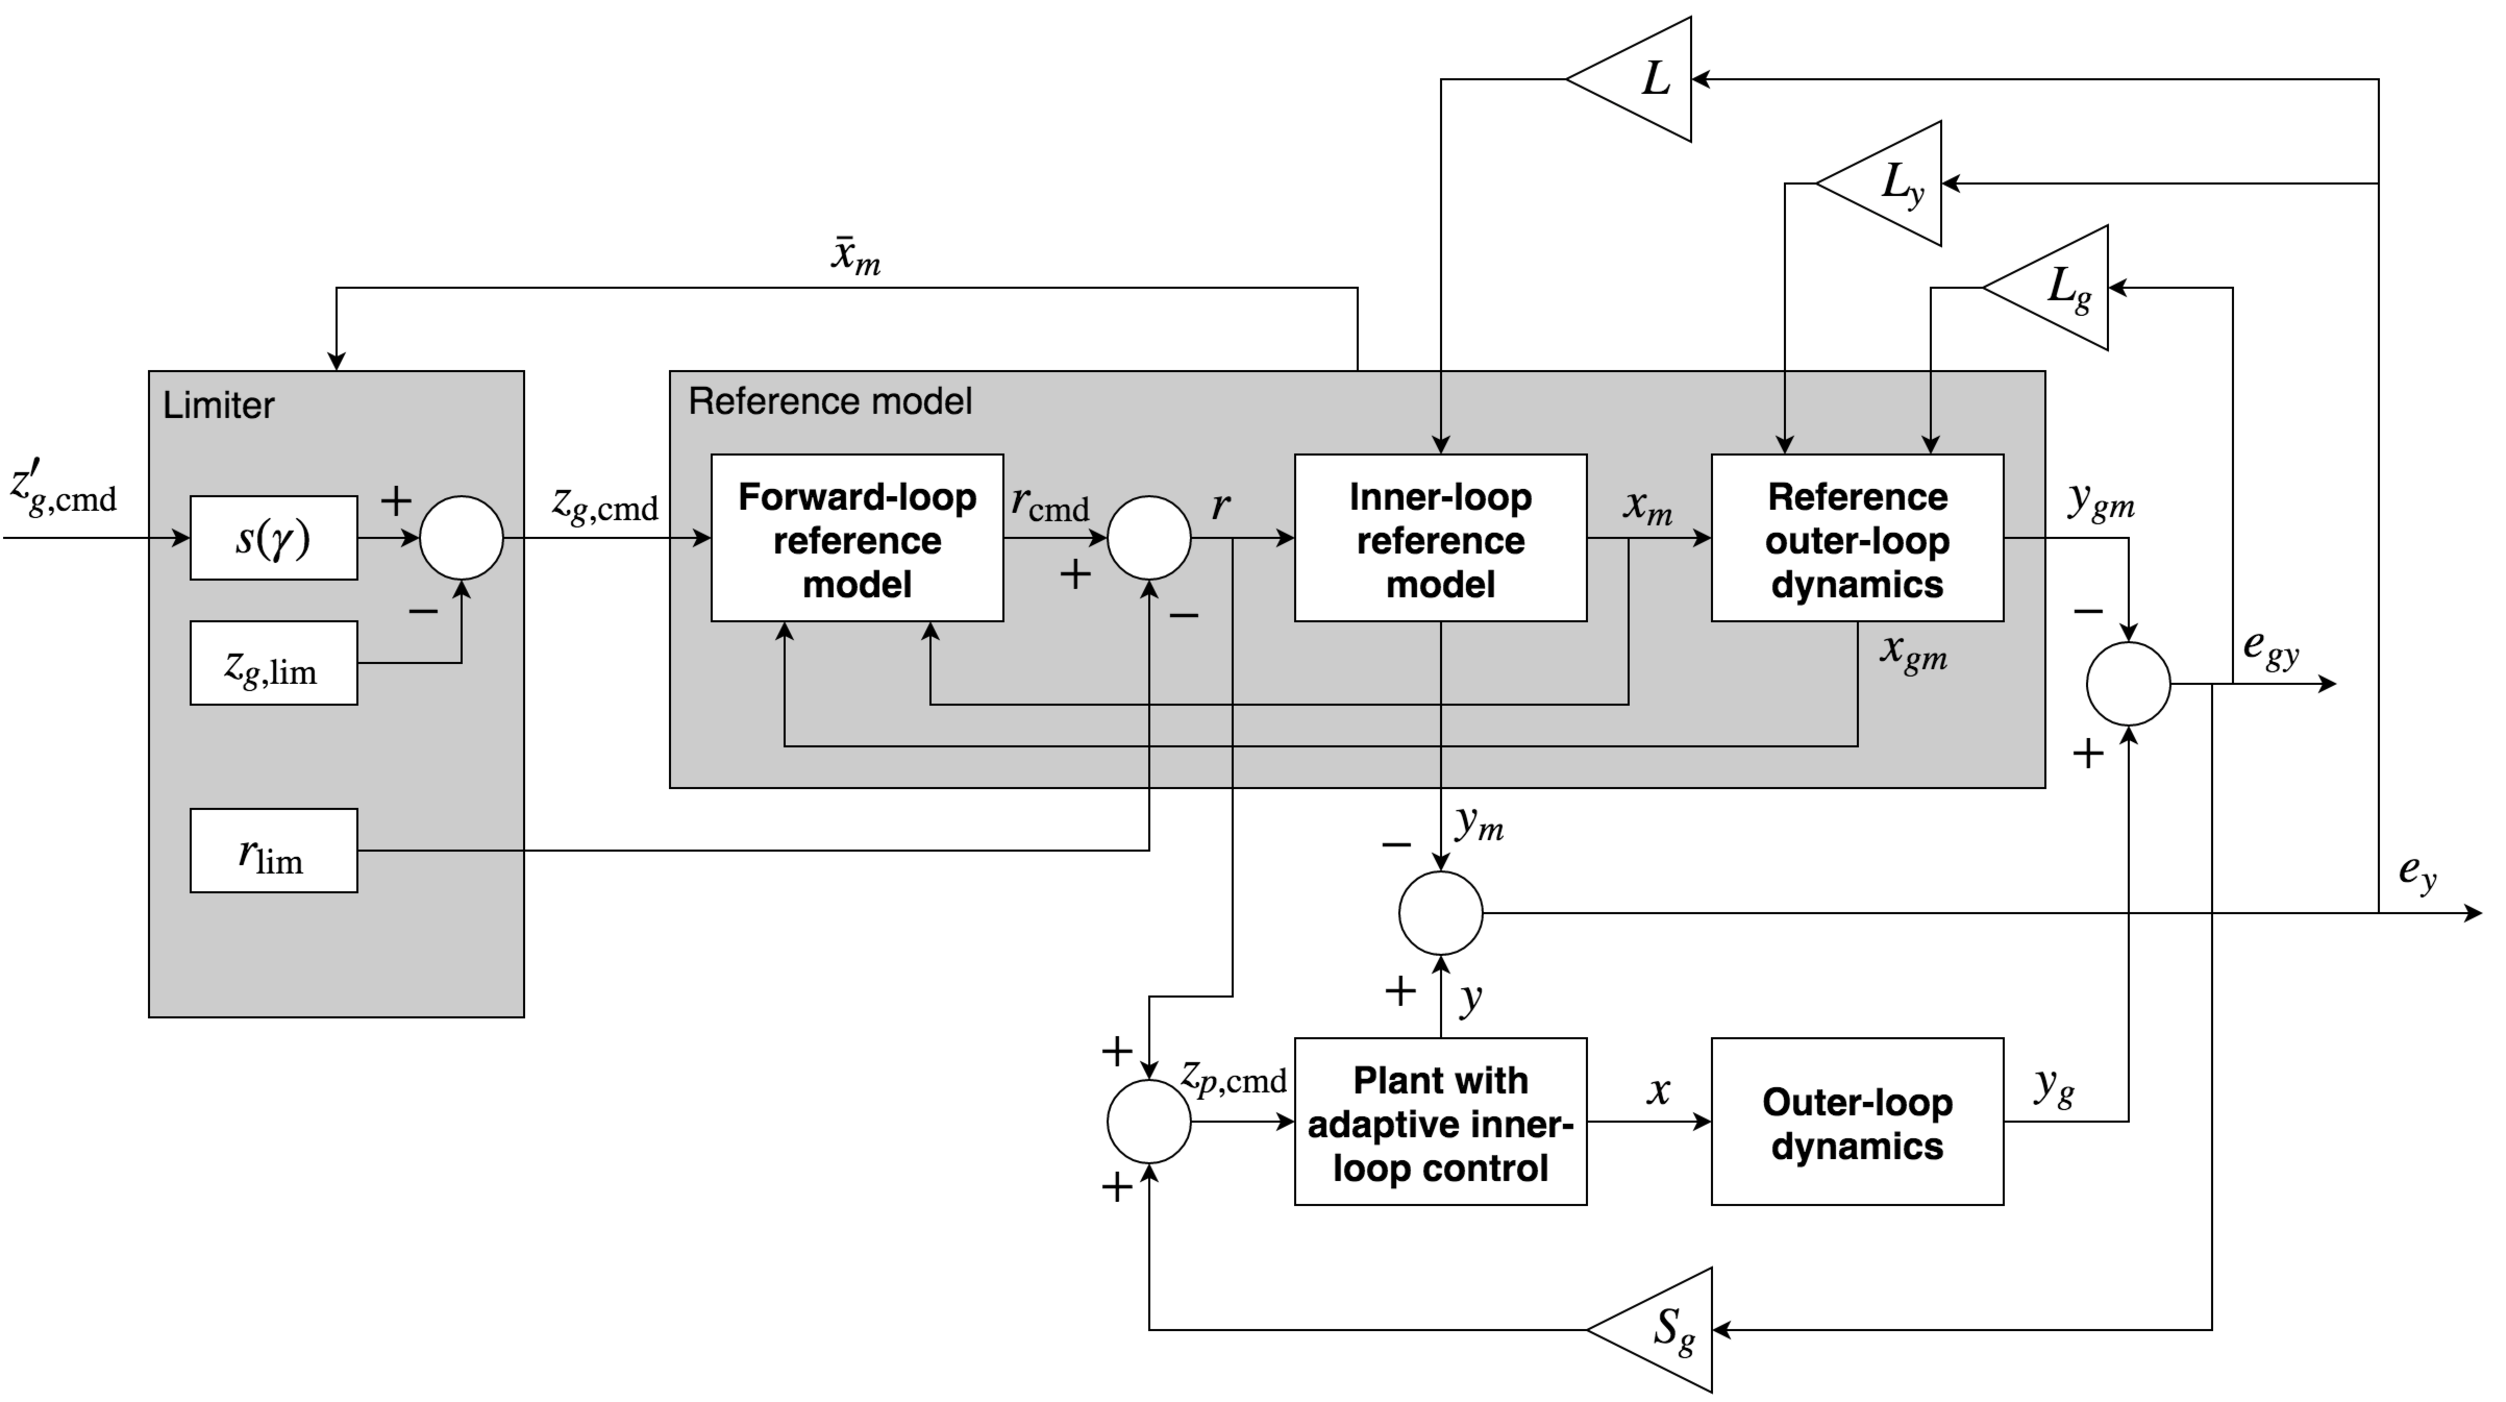
\includegraphics[width=3.0in]{\figurepath/block_limiter.pdf}
      \vspace{-0.1in}
      \caption{Expanded outer-loop block diagram with limiter.\label{fig.innerAndOuterLoopDansOutputFeedbackWithLimiter}}
    \end{center}
  \end{figure}

  Using the outer-loop command $z_{g,\text{cmd}}(t)$ as generated by\ \eqref{eqn.zcmdlimited} into\ \eqref{eqn.compactreferencemodel2} gives
  {%
    \small
    \begin{align}
      \label{eqn.compactrefmodelwithlimiter2}
      \dot{\bar{x}}_{m}(t)
      &=
      \bigr(\bar{A}_{m} + \bar{B}k_{r}\gamma(\bar{x}_{m}(t)) K_{\text{lim}} + \bar{B}_{m}\gamma(\bar{x}_{m}(t)) K_{\text{lim}}\bigr)\bar{x}_{m}(t) \nonumber \\
      & \qquad
      + \bar{B}_{m}\bigr(1-\gamma(\bar{x}_{m}(t))\bigr)z_{g,\text{cmd}}^{\prime}(t) \nonumber \\
      & \qquad
      - \bar{L}_{y}e_{y}(t) - \bar{L}_{g}e_{gy}(t) \\
      r_{\text{cmd}}(t)
      &=
      \bar{C}_{m}\bar{x}_{m}(t) \nonumber
    \end{align}
  }%


  \subsection{Stability}

  Because $r(t)$ and $z_{g,\text{cmd}}(t)$ do not appear in the error dynamics\ \eqref{eqn.innerAndOuterLoopErrorDynamics1}, the state-limiter modification does not require any change to the Lyapunov function in\ \eqref{eqn.lyapfunction_2} to prove boundedness of the errors $e_{x}(t)$ and $e_{g}(t)$.
  However, in the stability proof without the state limiter, the boundedness of $z_{g,\text{cmd}}(t)$, $e_{y}(t)$, and $e_{gy}(t)$ and stability of $\bar{A}_{m}$ in\ \eqref{eqn.compactreferencemodel} imply boundedness of the reference model states $x_{m}(t)$, $x_{gm}(t)$, and $x_{fm}(t)$, from which boundedness of the plant states $x(t)$ and $x_{g}(t)$ is concluded.
  However, showing boundedness of the reference model states is less obvious when using the state limiter, which modifies the entire reference model dynamics in\ \eqref{eqn.compactreferencemodel} to obtain the limited reference model dynamics in\ \eqref{eqn.compactrefmodelwithlimiter2}.
  Thus it is necessary to ensure that with the limiting modifications the reference model state $\bar{x}_{m}(t)$ is still bounded, and global stability is still proved, as stated in the following theorem.

  \begin{thm-dan}\label{thm.outerlooplimiter}
    The uncertain system in\ \eqref{eqn.wholeSystemUncertain} with inner-loop controller specified by the control law in\ \eqref{eqn.u}, update law in\ \eqref{eqn.updatelaw}, and the reference model in\ \eqref{eqn.refmodelWithBd} where $S_{1}$ and $L$ are chosen as described in Section~\ref{sec.InnerLoopControlDesign}, and the outer-loop controller specified by the outer-loop reference model in\ \eqref{eqn.refmodelouter}, forward-loop reference model component in\ \eqref{eqn.forwardloopcontroller}, with inner-loop command input $z_{p,\text{cmd}}(t)$ is prescribed by\ \eqref{eqn.zpcmd} and\ \eqref{eqn.egs}, where $r(t)$ is given by\ \eqref{eqn.compactrefmodelwithlimiter2},\ \eqref{eqn.rrcmdrlim}, and\ \eqref{eqn.rlim}, and outer-loop command generated by\ \eqref{eqn.zcmdlimited},\ \eqref{eqn.sofgamma}, and\ \eqref{eqn.zglim}, with $S_{g}$, $L_{g}$, and $L_{y}$ selected as described above, results in global stability, with $\lim_{t\rightarrow\infty}e_{x}(t)=0$ and $\lim_{t\rightarrow\infty}e_{g}(t)=0$.
  \end{thm-dan}

  \begin{proof-dan}
    This proof follows from the proof of Theorem~\ref{thm.outerloop} by proposing the same candidate Lyapunov function as in\ \eqref{eqn.lyapfunction_2} and differentiating to obtain\ \eqref{eqn.outerlooplyapderivative} from which it can be concluded that $e_{x}(t), \; e_{g}(t) , \;\widetilde{\Theta}(t)\in\mathcal{L}_{\infty}$.
    Bounds on $e_{x}(t)$ and $e_{g}(t)$ can be found as follows
    \begin{equation}
      \label{eqn.boundaonexandeg}
      \begin{split}
        \|e_{x}(t)\|
        & \leq
        \sqrt{\frac{V(0)}{\lambda_{\text{min}}(P_{x})}} \\
        \|e_{g}(t)\|
        & \leq
        \sqrt{\frac{V(0)}{\lambda_{\text{min}}(P_{g})}}
      \end{split}
    \end{equation}
    giving the following bounds on their respective measured output errors $e_{y}(t)$ and $e_{gy}(t)$ as
    \begin{equation}
      \label{eqn.boundaoneyandegy}
      \begin{split}
        \|e_{y}(t)\|
        & \leq
        e_{y,\text{max}}
        =
        \|C\|
        \sqrt{\frac{V(0)}{\lambda_{\text{min}}(P_{x})}} \\
        \|e_{gy}(t)\|
        & \leq
        e_{gy,\text{max}}
        =
        \|C_{g}\|
        \sqrt{\frac{V(0)}{\lambda_{\text{min}}(P_{g})}}
      \end{split}
    \end{equation}
    Propose the following additional candidate Lyapunov function to prove boundedness of the reference model state
    \begin{equation}
      \label{eqn.Lyapxmbar}
      \bar{V}\bigr(\bar{x}_{m}(t)\bigr) = \bar{x}_{m}^{\top}(t)\bar{P}\bar{x}_{m}(t)
    \end{equation}
    Differentiating\ \eqref{eqn.Lyapxmbar} gives
    \begin{equation}
      \label{eqn.Lyapxmbardot1}
      \dot{\bar{V}}\bigr(\bar{x}_{m}(t)\bigr)
      =
      \dot{\bar{x}}_{m}^{\top}(t)\bar{P}\bar{x}_{m}(t)
      + \bar{x}_{m}^{\top}(t)\bar{P}\dot{\bar{x}}_{m}(t)
    \end{equation}
    Using $\bar{Q}$ from\ \eqref{eqn.LyapEqnPbar} and defining the following
    \begin{equation}
      \label{eqn.qbarlim}
      \bar{Q}_{\rm{\lim}}(\gamma)
      =
      2\bar{P}(\bar{B}_{m}+\bar{B}k_{r})R_{\text{lim}}^{\top}\gamma (k_{r}^{\top}\bar{B}^{\top}+\bar{B}_{m}^{\top})\bar{P}
      \geq
      0
    \end{equation}
    allowing\ \eqref{eqn.Lyapxmbardot1} to be rewritten as
    \begin{equation}
      \label{eqn.vbardot}
      \begin{split}
        &
        \dot{\bar{V}}\bigr(\bar{x}_{m}(t)\bigr)
        =
        -\bar{x}_{m}^{\top}(\bar{Q}+\bar{Q}_{\rm{\lim}}(\gamma))\bar{x}_{m}(t) \\
        & \qquad
        + 2\bar{x}_{m}^{\top}(t)\bar{P}\bigr(\bar{B}_{m}(1-\gamma)z_{g,\text{cmd}}^{\prime}(t) \\
        & \qquad
        - \bar{L}_{y}e_{y}(t) - \bar{L}_{g}e_{gy}(t)\bigr)
      \end{split}
    \end{equation}
    Note that the bounds on $e_{y}(t)$ and $e_{gy}(t)$ in\ \eqref{eqn.boundaoneyandegy} are independent of $\bar{x}_{m}(t)$.
    Eq.\ \eqref{eqn.vbardot} contains a negative quadratic term in $\bar{x}_{m}(t)$, and a sign indefinite term which is linear in $\bar{x}_{m}(t)$.
    Thus, for sufficiently large $\bar{x}_{m}(t)$, the derivative $\dot{\bar{V}}\bigr(x_{m}(t)\bigr)$ in\ \eqref{eqn.vbardot} becomes strictly negative.
    This is quantified precisely by the following statement: $\dot{\bar{V}}\bigr(\bar{x}_{m}(t)\bigr)<0$ outside the compact set

    \begin{widetext}
      \vspace{0.2in}
      \begin{equation}
        \label{eqn.limiterCompactSet}
        E_{\delta}=
        \biggr\{%
        \bar{x}_{m}(t)\in\mathbb{R}^{n} \; : \;
        \|\bar{x}_{m}(t)\|
        \leq
        \frac{2\lambda_{\text{max}}(\bar{P})\bigr(
        \|\bar{B}_{m}\|(1-\gamma)z_{g,\text{cmd,max}}^{\prime}+
        \|\bar{L}_{y}\|e_{y,\text{max}}+\|\bar{L}_{g}\|e_{gy,\text{max}}
        \bigr)}{\lambda_{\text{min}}(\bar{Q}+\bar{Q}_{\text{lim}}(\gamma))}
        \biggr\} \\[12pt]
      \end{equation}
      \noindent\makebox[\linewidth]{\rule{\textwidth}{0.2pt}}
      \vspace{-0.3in}
    \end{widetext}
    for all $\gamma(\bar{x}_{m}(t))\in[0,1]$.
    Thus the entire reference model state $\bar{x}_{m}(t)$ is bounded\ \cite{narendra.stable.2005} which, with the boundedness of the errors $e_{x}(t)$ and $e_{g}(t)$, implies that $x(t),\;x_{g}(t)\in\mathcal{L}_{\infty}$.
    With this, it can be concluded using Barbalat's Lemma\ \cite{narendra.stable.2005} that $\lim_{t\rightarrow\infty}e_{x}(t)=0$ and $\lim_{t\rightarrow\infty}e_{g}(t)=0$.
  \end{proof-dan}

  In the absence of the state limiter, satisfaction of the control goal of outer-loop command tracking was discussed in Corollary~\ref{cor.zgcmdtracking}.
  When using the state limiter, Theorem~\ref{thm.outerloop}, like Theorem~\ref{thm.outerlooplimiter}, provided $z_{g}(t)\rightarrow z_{gm}(t)$ as $t\rightarrow\infty$.
  However, without the limiter, the reference model in\ \eqref{eqn.compactreferencemodel} produced $z_{gm}(t)$ that was a filtered version of $z_{g,\text{cmd}}^{\prime}(t)$.
  When using the limiter this is no longer true; $z_{gm}(t)$ is the output of\ \eqref{eqn.compactrefmodelwithlimiter2}.
  Thus asymptotic tracking of $z_{g,\text{cmd}}^{\prime}(t)$ by $z_{g}(t)$ doesn't hold in general.
  However, if a desired outer-loop command $z_{g,\text{cmd}}^{\prime}(t)$ is given such that the limiter is inactive and $\gamma\bigr(\bar{x}_{m}(t)\bigr)=0$, the same conclusion as in Corollary~\ref{cor.zgcmdtracking} can be made, with $z_{g,\text{cmd}}(t) = z_{g,\text{cmd}}^{\prime}(t)$.
  This statement is formalized in the following corollary to Theorem~\ref{thm.outerlooplimiter}.

  \begin{cor-dan}\label{cor.notForcingLimiting}
    For all piecewise constant outer-loop command inputs $z_{g,\text{\rm{cmd}}}^{\prime}(t)$ which satisfy $\|z_{g,\text{\rm{cmd}}}^{\prime}(t)\|_{\infty}\leq z_{g,\text{\rm{cmd,max}}}^{\prime}$, the outer-loop regulated output $z_{g}(t)$ tracks $z_{g,\text{\rm{cmd}}}^{\prime}(t)$ asymptotically, where $z_{g,\text{\rm{cmd,max}}}^{\prime}$ is given by
    \begin{equation}
      \label{eqn.zgcmdprimemax}
      z_{g,\text{\rm{cmd,max}}}^{\prime}
      =
      \frac{\bar{x}_{m,\text{\rm{max}}}}{\|h_{m}\|_{1}}
    \end{equation}
    where $h_{m}$ is the impulse response of the nominal reference model, given by\ \eqref{eqn.compactrefmodelwithlimiter2} with $\gamma(\bar{x}_{m}(t))=0$, $\bar{L}_{y}=0$ and $\bar{L}_{g}=0$, and $\bar{x}_{m,\text{\rm{max}}}=\text{\rm{max}}_{\bar{x}_{m}(t)\in\Omega_{\delta}}\|\bar{x}_{m}(t)\|$.
  \end{cor-dan}

  \begin{proof-dan}
    For all $\bar{x}_{m}(t)\in\Omega_{\delta}$ the state limiter is inactive, and the evolution of the reference model state $\bar{x}_{m}(t)$ is governed by\ \eqref{eqn.compactrefmodelwithlimiter2} with $\gamma(\bar{x}_{m}(t))=0$, while $e_{y}(t)$ and $e_{gy}(t)$ tend to zero asymptotically.
    Thus, the reference model state $\bar{x}_{m}(t)$ ultimately depends only on the command input $z_{g,\text{cmd}}^{\prime}(t)$.
    The following bound on the reference model state holds, where $h_{m}$ is the impulse response of the nominal reference model,\ \eqref{eqn.compactrefmodelwithlimiter2} with $\gamma(\bar{x}_{m}(t))=0$.
    \begin{equation*}
      \|\bar{x}_{m}(t)\|_{\infty}=\bar{x}_{m,\text{max}} \leq \|h_{m}\|_{1}\|z_{g,\text{cmd}}^{\prime}(t)\|_{\infty}
    \end{equation*}
    From this, the bound $z_{g,\text{\rm{cmd,max}}}^{\prime}$ that ensures the reference model state $\bar{x}_{m}(t)\in\Omega_{\delta}$, thus not invoking the state limiter, and providing the tracking properties given in Corollary~\ref{cor.zgcmdtracking}.
  \end{proof-dan}

  \begin{rem-dan}
    Corollary~\ref{cor.notForcingLimiting} states that if the desired outer-loop command $z_{g,\text{cmd}}^{\prime}(t)$ is such that the system is not driven to enter the limiting region, that the limiter will not impact tracking performance of the system.
    This is due to the fact that the convergence of the tracking errors $e_{y}(t)$ and $e_{gy}(t)$ to zero is obtained regardless of whether the limiter is invoked or not.
    In other words, as these errors tend to zero, only the desired outer-loop command $z_{g,\text{cmd}}^{\prime}(t)$ can drive the reference model state $\bar{x}_{m}(t)$ out of $\Omega_{\delta}$, as governed by\ \eqref{eqn.compactreferencemodel}.
    Thus, if the desired outer-loop command is such that it does not force $\bar{x}_{m}(t)$ outside of $\Omega_{\delta}$, the limiter will become inactive.
    Corollary~\ref{cor.notForcingLimiting} then finds the maximum value of $z_{g,\text{cmd}}^{\prime}(t)$ such that $\bar{x}_{m}(t)\in\Omega_{\delta}$ using the impulse response of the reference model.
  \end{rem-dan}

  \begin{rem-dan}
    The benefits of the state limiter are apparent from the compact set in\ \eqref{eqn.limiterCompactSet} outside of which $\dot{\bar{V}}(\bar{x}_{m}(t))<0$.
    The size of $E_{\delta}$ monotonically decreases in size as $\gamma(\bar{x}_{m}(t))$ increases, hence shrinking the bound on $\bar{x}_{m}(t)$ when the limiter is invoked, versus without the limiter.
  \end{rem-dan}

  \subsubsection{Degrees of Freedom}

  The limiter described above has several degrees of freedom which can be chosen by the designer to achieve the desired performance.
  These degrees of freedom are the gains $k_{r}$, $R_{\text{lim}}$, $\bar{Q}$, and the modulation function $\gamma(\bar{x}_{m}(t))$ and the corresponding sets $\Omega$ and $\Omega_{\delta}$.
  The limiter components $r_{\text{lim}}(t)$ and $z_{g,\text{lim}}(t)$ enter through the input matrices $\bar{B}$ and $\bar{B}_{m}$, respectively, of the reference model in\ \eqref{eqn.compactreferencemodel2}.
  The matrix $R_{\text{lim}}$ scales $K_{\text{lim}}$ in\ \eqref{eqn.Klim}, which is the gain used in both of the limiting components $r_{\text{lim}}(t)$ and $z_{g,\text{lim}}(t)$, whereas $k_{r}$ scales only $r_{\text{lim}}(t)$.
  Thus, by adjusting $R_{\text{lim}}$ and $k_{r}$, the relative influence of the limiter through $\bar{B}$ and $\bar{B}_{m}$ can be changed.
  This alters the the effective reference model matrix in\ \eqref{eqn.compactrefmodelwithlimiter2} when the limiter becomes active, and thus $\bar{Q}_{\rm{\lim}}(\gamma(\bar{x}_{m}(t)))$ in\ \eqref{eqn.qbarlim}.
  This, along with the matrix $\bar{Q}$, alters the region outside of which $\dot{\bar{V}}<0$, and thus affects the time response of the system when the state limiter is active.
  With $k_{r}=0$ and $R_{\text{lim}}=0$ the limiter would still be stable, however the only adjustment would come through the reduction of the outer-loop command $z_{g,\text{cmd}}^{\prime}(t)$ in\ \eqref{eqn.vbardot}.
  The modulation function $\gamma(\bar{x}_{m}(t))$ simply defines based on $\bar{x}_{m}$ when the limiter becomes active, and can be selected so as to depend on the various elements of $\bar{x}_{m}(t)$ as desired.

  \subsection{Complete Controller Summary with Limiter}

  The uncertain plant\ \eqref{eqn.uncsystemWithBd}, outer-loop dynamics\ \eqref{eqn.outerLoopDynamics}, inner-loop reference model\ \eqref{eqn.refmodelWithBd}, outer-loop reference model\ \eqref{eqn.refmodelouter}, forward-loop reference model component\ \eqref{eqn.forwardloopcontroller}, inner-loop command\ \eqref{eqn.zpcmd},\ \eqref{eqn.egs},\ \eqref{eqn.rrcmdrlim} and\ \eqref{eqn.rlim}, outer-loop command\ \eqref{eqn.zcmdlimited},\ \eqref{eqn.sofgamma}, and\ \eqref{eqn.zglim}, control law\ \eqref{eqn.u}, and update law\ \eqref{eqn.updatelaw} are summarized as follows.

  {%
    \small
    \begin{equation*}
      \begin{aligned}
        \textbf{Plant:}
        && \dot{x}(t) &= Ax(t) + B\bigr(\Lambda u(t) + \Psi^{\top}x(t)\bigr) \\
        &&& \qquad
        + B_{\text{cmd}}z_{p,\text{cmd}}(t) + B_{d}x_{g}(t) \\
        && \dot{x}_{g}(t) &= A_{g}x_{g}(t) + B_{g}x(t) \\
        \textbf{Reference model:}
        && \dot{x}_{m}(t) &= A_{m}x_{m}(t) + B_{\text{cmd}}r(t) \\
        &&& \qquad
        - Le_{y}(t) + B_{d}x_{gm}(t) \\
        && \dot{x}_{gm}(t) &= B_{g}x_{m}(t) + A_{g}x_{gm}(t) \\
        &&& \qquad
        - L_{y}e_{y}(t) - L_{g}e_{gy}(t) \\
        && \dot{x}_{fm}(t) &= B_{f3}x_{m}(t) + B_{f2}x_{gm}(t) \\
        &&& \qquad
        + A_{fm}x_{fm}(t) + B_{f1}z_{g,\text{cmd}}(t) \\
        \textbf{Command:}
        && r_{\text{cmd}}(t) &= C_{fm}x_{fm}(t) + D_{f1}z_{g,\text{cmd}}(t) \\
        &&& \qquad
        + D_{f2}x_{gm}(t) + D_{f3} x_{m}(t) \\
        && r(t) &= r_{\text{cmd}}(t) - r_{\text{lim}}(t) \\
        && r_{\text{lim}}(t) &= -k_{r}\gamma\bigr(\bar{x}_{m}(t)\bigr) K_{\text{lim}}\bar{x}_{m}(t) \\
        && z_{g,\text{cmd}}(t) &= s(\gamma)z_{g,\text{cmd}}^{\prime}(t) - z_{g,\text{lim}}(t) \\
        && z_{p,\text{cmd}}(t) &= r(t) + S_{g}e_{gy}(t) \\
        \textbf{Errors:}
        && e_{y}(t) &= C\bigr(x(t)-x_{m}(t)\bigr) \\
        && e_{gy}(t) &= C_{g}\bigr(x_{g}(t) - x_{gm}(t)\bigr) \\
        \textbf{Control:}
        && u(t) &= \bigr(K_{x}+\Theta(t)\bigr)^{\top}x_{m}(t) \\
        && \dot{\Theta}(t) &= -\Gamma x_{m}(t)\bigr(S_{1}e_{y}(t)\bigr)^{\top}\text{sgn}(\Lambda) \\
      \end{aligned}
    \end{equation*}
  }\\[-32pt]

  \section{Simulation Results}

  This section contains simulations comparing the performance of the baseline and adaptive controller, as well as the state limiter, on the nonlinear 6-DOF Generic Hypersonic Vehicle model\ \cite{wiese.adaptive.2013, rollins.nonlinear.2013, wiese.gnc.2015, wiese.jgcd.2015}.
  The equations of motion were linearized about a Mach 5 flight condition at an altitude of 80,000 feet.
  Modal analysis was then used to decouple the linearized equations of motion into three reduced order subsystems consisting of the first-order velocity, fourth-order longitudinal, and fifth-order lateral-directional dynamics.
  This allowed three decoupled controllers to be designed: a velocity controller with single loop, and controllers for the longitudinal and lateral-directional subsystems with both inner and outer loops, as described above.
  The longitudinal subsystem inner-loop state variables are angle-of-attack and pitch rate, with the outer-loop state variables pitch angle and altitude.
  The lateral-directional inner-loop state variables are sideslip angle, roll rate, and yaw rate, with outer-loop state variables roll angle and heading angle.
  Uncertainty consisting of control effectiveness on all surfaces reduced to 20\% of the nominal value, center-of-gravity shifted 0.7 feet rearward, and the rolling moment coefficient $C_{l}$ reduced to 10\% of the nominal value is considered.
  The performance of the nominal baseline controller is compared to that of the adaptive controller both with and without the state limiter, for a heading change of 5 degrees, on the nonlinear, uncertain GHV model.
  For each subsystem $\Psi_{\text{max}}$ in Assumption~\ref{ass.plant}\ref{ass.p.unc}-\ref{ass.p.unc.wp} was selected by acknowledging physical constraints of the plant.
  For example, the center-of-gravity must lie within the physical extents of the vehicle, and values of aerodynamic coefficients are bounded based on the flight envelop as determined by the propulsive and structural limitations of the vehicle.

  Figure~\ref{fig.baselineUncertainLatrState} shows that the baseline controller is not able to maintain stability when applied to the uncertain vehicle model.
  In this figure, both the reference and plant state can seen be seen to be diverging, showing the instability caused by the introduction of the uncertainty, and demonstrating a case in which an adaptive controller can be used to stabilize the uncertain system.
  Figure~\ref{fig.adaptiveUncertainLatrState} shows the response of the uncertain plant with the adaptive controller summarized in Sec.~\ref{sec.outerLoopDesignProcedureSummary}.
  In this case, the adaptive controller is able to accommodate the uncertainty and maintain stability, but with large oscillations and sideslip angle occuring, both of which are undesirable.
  Figure~\ref{fig.stateLimiterState} shows the response of the uncertain plant with adaptive controller and limiter as described in Sec.~\ref{sec.outerLoop.stateLimiting} used to suppress the large oscillations in sideslip.
  Here, the modulation function $\gamma(\bar{x}(t))$ as described in Ref.\ \cite{lavretskywise.book.2013} in\ \eqref{eqn.zglim}\ \eqref{eqn.rlim} is chosen only as a function of sideslip angle, and the constraints on sideslip as given by $\Omega$ set at 0.2 degrees.
  In this case the adaptive controller not only maintains stability, but the use of the limiter confines the oscillations in sideslip angle to a maximum magnitude of less than 0.2 degrees as desired.

  \begin{figure}[H]
    \hspace{-0.2in}
    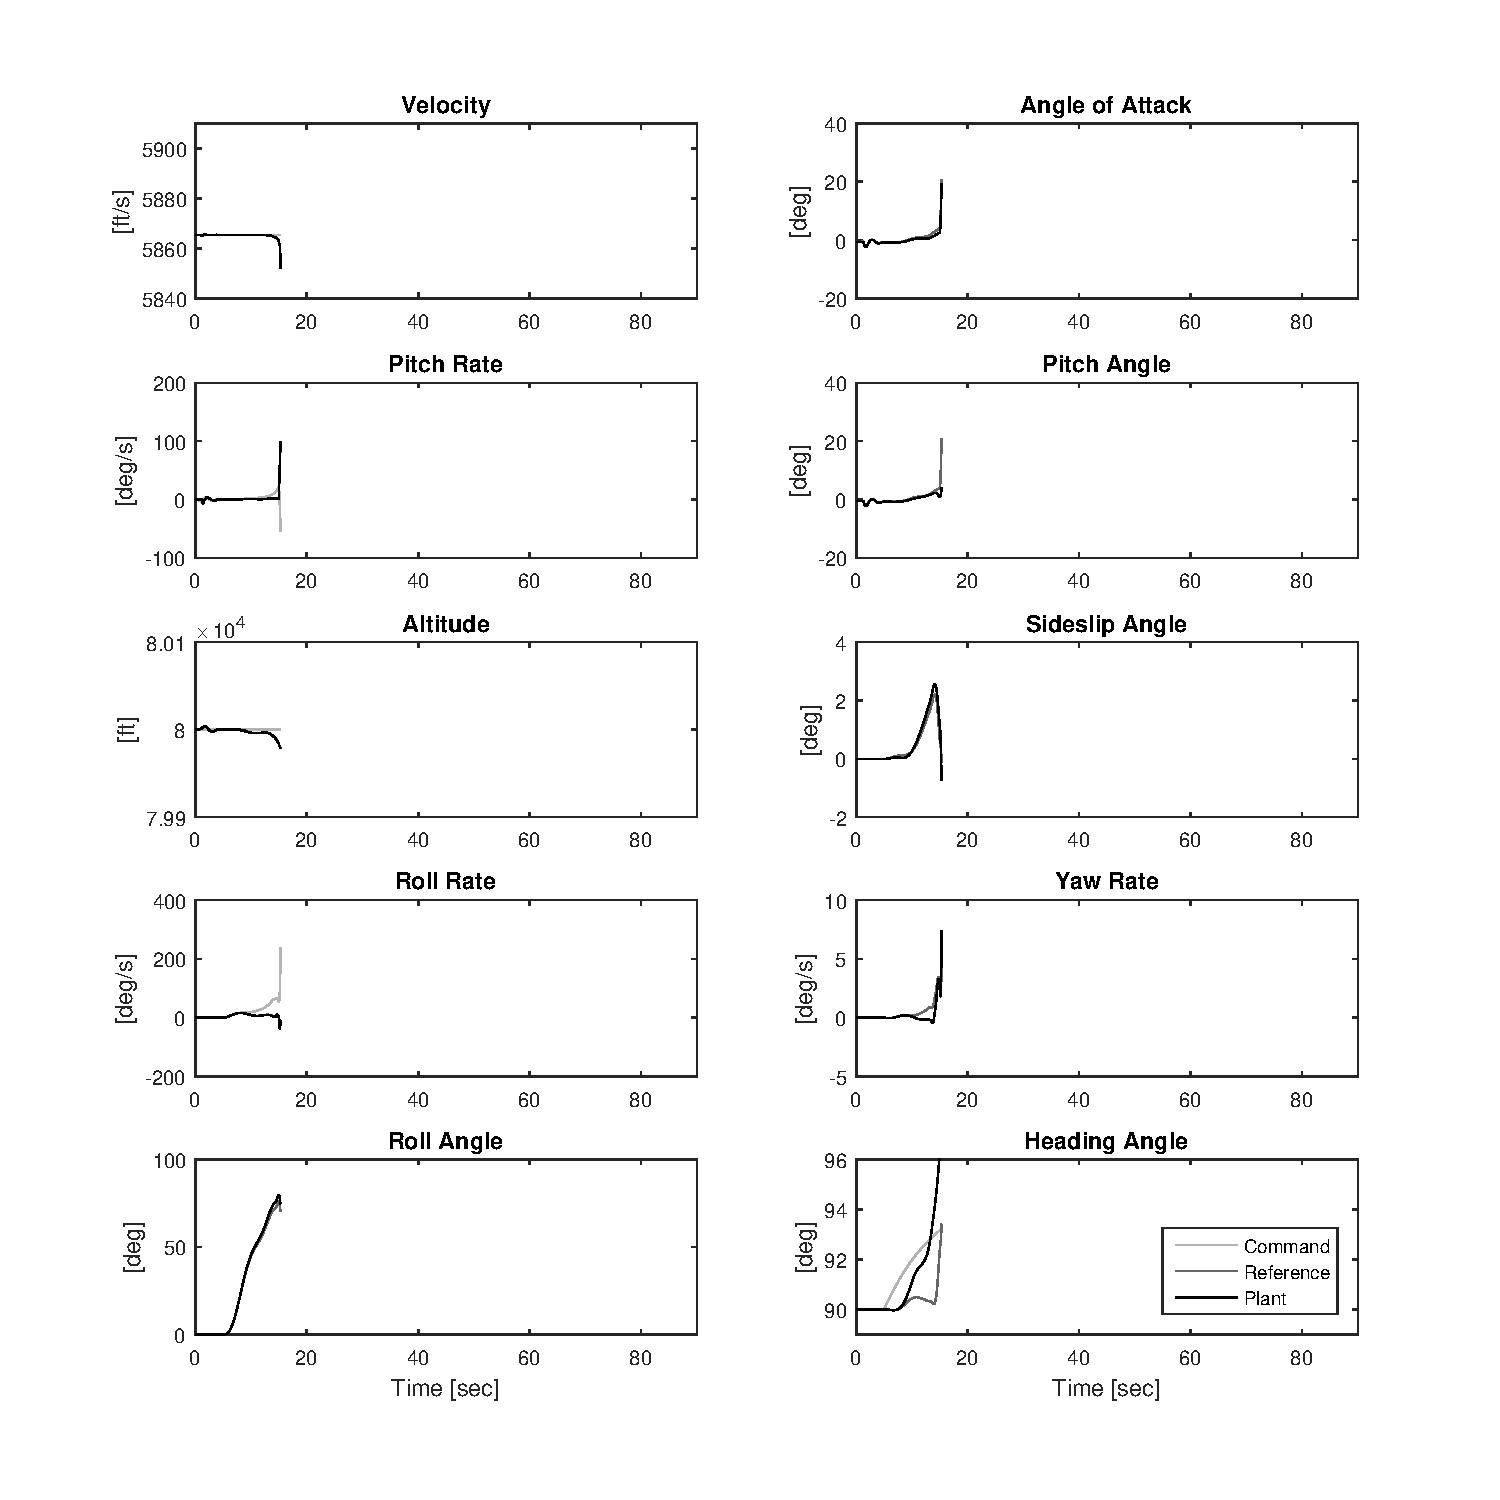
\includegraphics[width=3.6in]{\figurepath/baseline.pdf}
    \vspace{-0.5in}
    \caption{Plant states for baseline controller applied to uncertain plant in response to a 5 degree heading turn.\label{fig.baselineUncertainLatrState}}
  \end{figure}

  \begin{figure}[H]
    \hspace{-0.2in}
    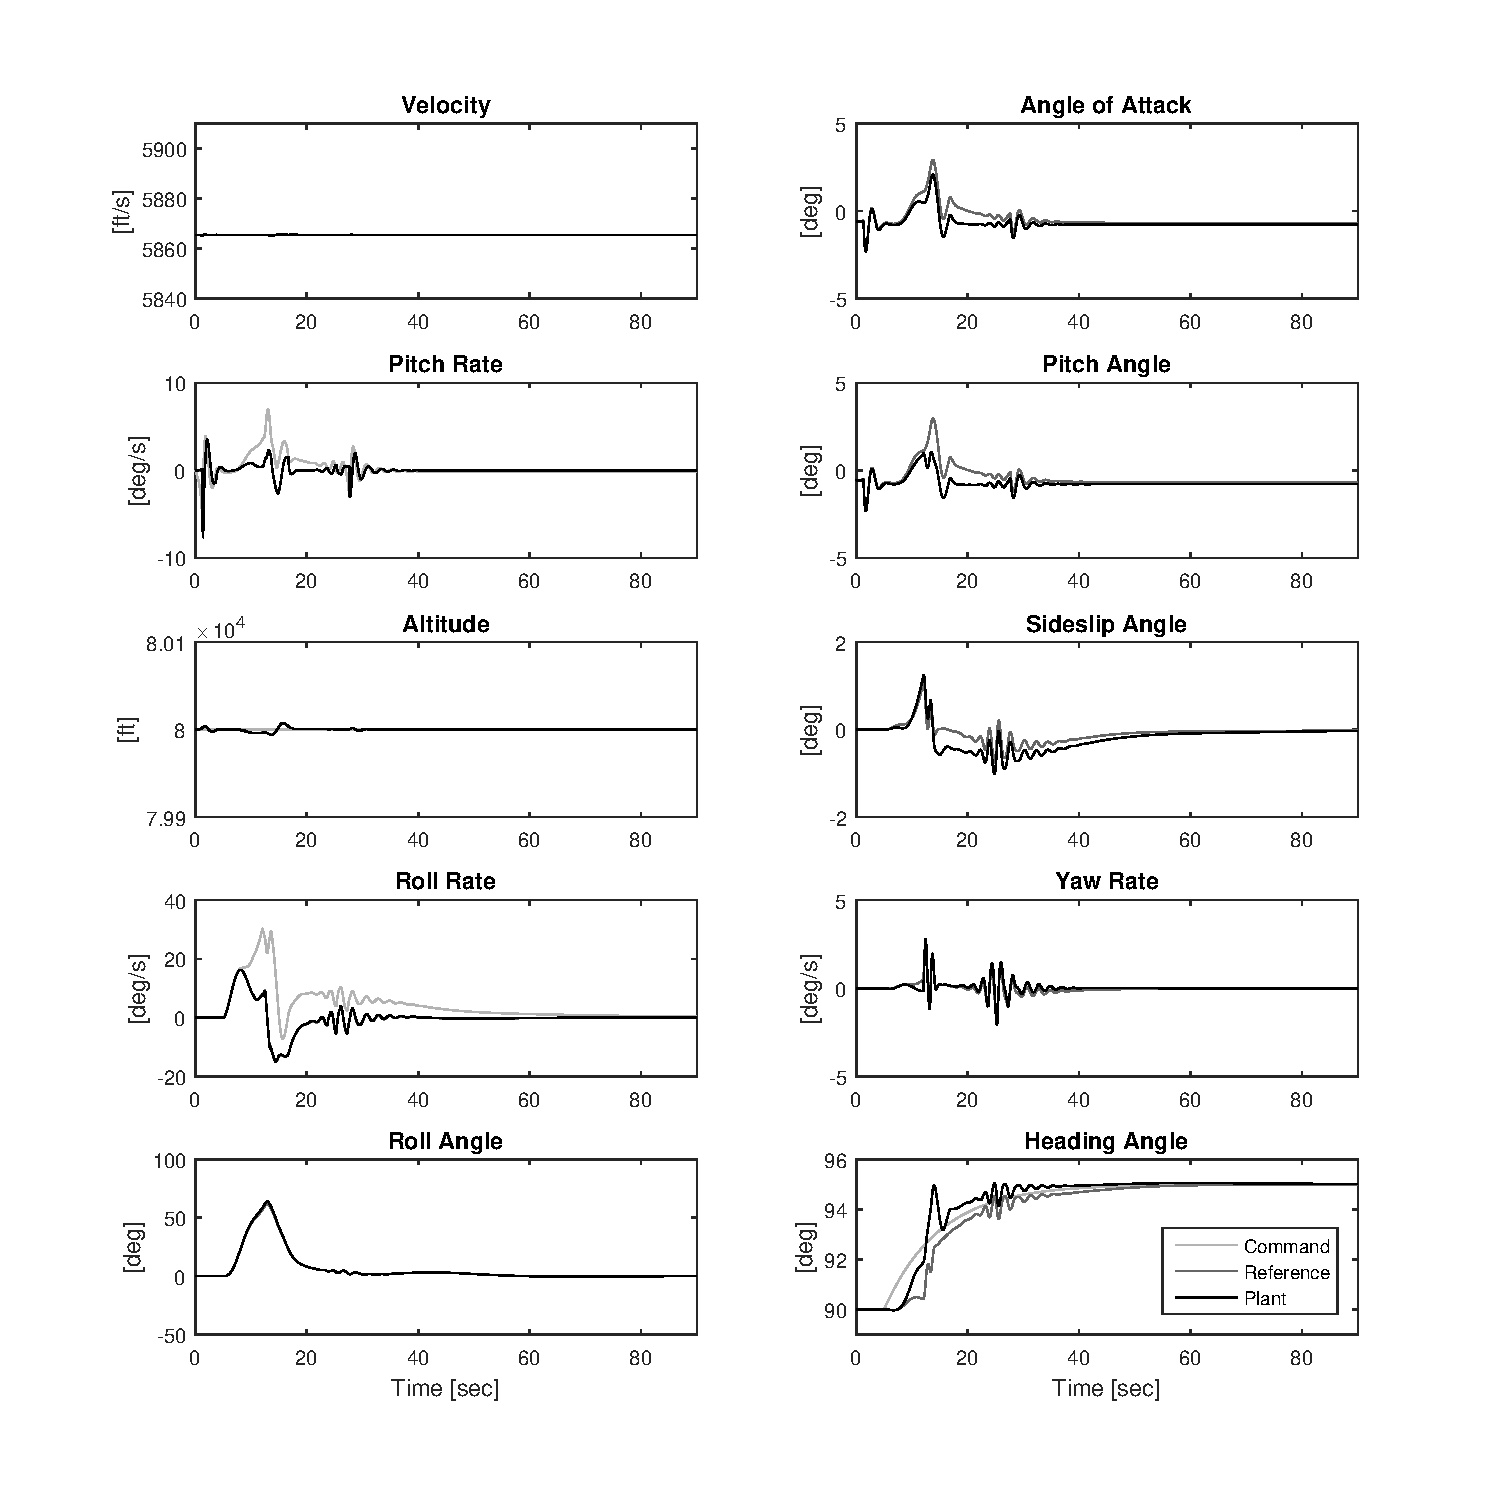
\includegraphics[width=3.6in]{\figurepath/adaptive.pdf}%\}
    \vspace{-0.4in}
    \caption{Plant states for adaptive controller applied to uncertain plant in response to a 5 degree heading turn.\label{fig.adaptiveUncertainLatrState}}
  \end{figure}

  \begin{figure}[H]
    \hspace{-0.2in}
    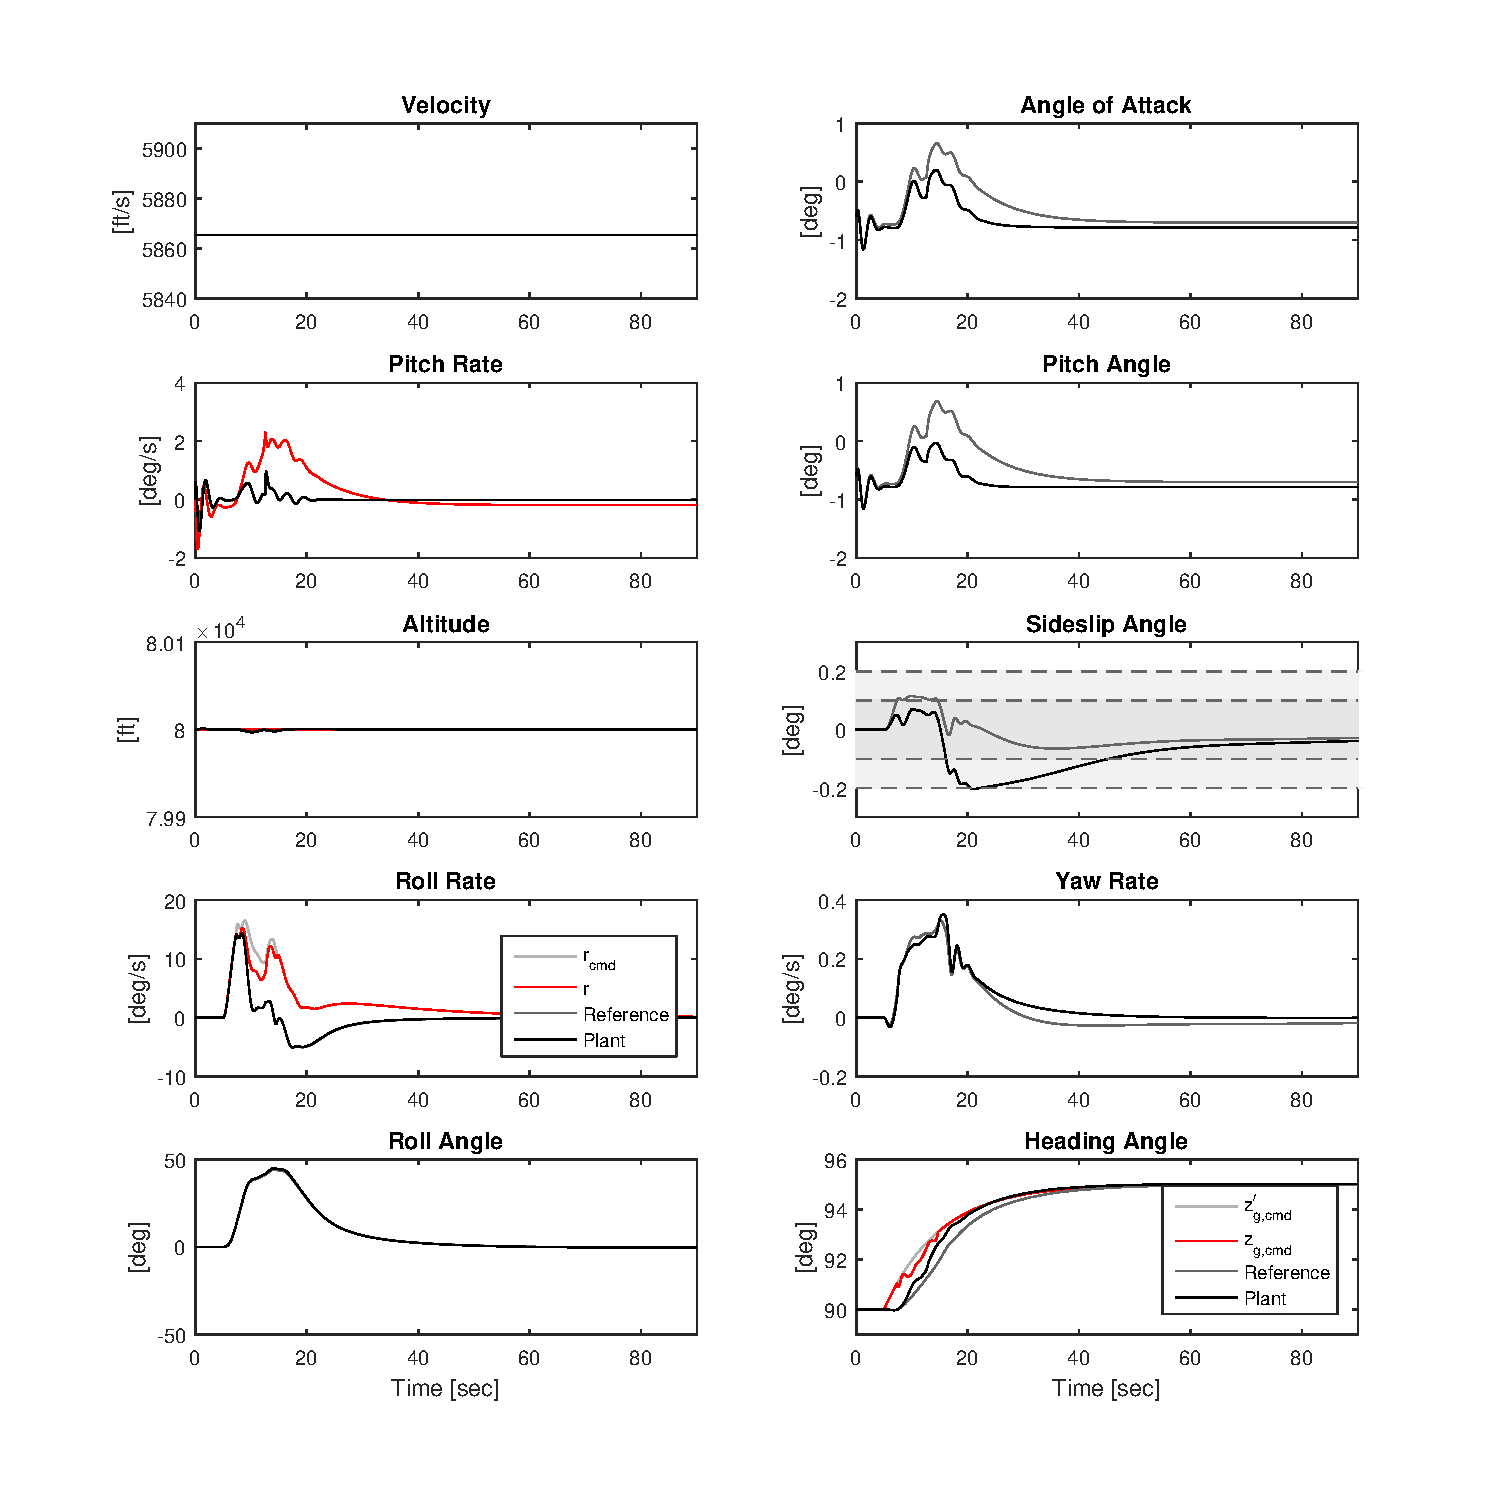
\includegraphics[width=3.6in]{\figurepath/limiter.pdf}%\}
    \vspace{-0.3in}
    \caption{Plant states for adaptive controller applied to uncertain plant in response to a 5 degree heading turn with sideslip angle Limiter.\label{fig.stateLimiterState}}
  \end{figure}

  \section*{Acknowledgment}
  This research is funded by the Universal Technology Corporation (UTC) contract FA8650--10--D--3037 subcontract agreement 15--S2606--04--C19 for Adaptive Flight Control for Hypersonic Vehicles with Integrated Loops.

  \bibliographystyle{\bibstylepath}
  \bibliography{\bibsourcepath}

  % Provides some padding at end of references
  \onecolumn
  \begin{multicols}{2}
  \newpage
  \end{multicols}

\end{document}
